\section{Experimental Setup}
\label{app:exp_details}

\paragraph{Multilingual setup}
For each combination of model size and pool size, we sweep $h$ over a fine grid of 19--27 values (see Table~\ref{tab:exp_setup} for a summary), with denser sampling at low repetition levels where the loss landscape changes most rapidly. The grid spans number of repetitions from below 1 to above 30, though configurations where the resulting $h$ exceeds 1 are excluded.
For larger models, the feasible range of $h$ is narrower because the longer training duration ($100 \times N$ tokens) produces higher repetition at the same $h$; for example, the 539M model on the 50M pool covers $r$ up to approximately 20.
Evaluation is performed on 10,000 samples from held-out test sets of both FineWeb2 (target language) and FineWeb (English), allowing us to measure both target-domain and generic-domain loss at each checkpoint.

\paragraph{Multi-domain setup}
For the three-domain experiments (Section~\ref{sec:multi_domain}), we train 101M models with a total training budget of 30B tokens (approximately $300 \times N$), increased relative to the bilingual setup to allow sufficient repetition of both target domains.
The three pool-size configurations correspond to: 5$\times$less (Wiki 20M, peS2o 100M), base (Wiki 100M, peS2o 500M), and 5$\times$more (Wiki 500M, peS2o 2.5B).
We sweep over total target fractions $h_{\text{total}} = h_{\text{wiki}} + h_{\text{peS2o}}$ ranging from 0.02 to 0.60 with step 0.02, under both equal weighting ($h_{\text{wiki}} = h_{\text{peS2o}}$) and proportional weighting ($h_{\text{wiki}} / h_{\text{peS2o}} = D_{\text{wiki}} / D_{\text{peS2o}}$).

\paragraph{Math setup}
For the OpenWebMath experiments, we sweep $h$ over a linear grid whose density depends on pool size: 26 values for the 10M and 100M pools and 8 values for the 1B pool (60 total per model size). The 805M model uses a denser grid (35, 35, and 20 values for the 10M, 100M, and 1B pools respectively; 90 total), because its longer training horizon (1M vs.\ 200K steps) produces higher repetition counts that require finer resolution.
The $h$ range is adapted to each pool size, spanning up to $h = 0.078$ for the 10M pool, $h = 0.78$ for the 100M pool, and $h = 1.0$ for the 1B pool.
The maximum number of repetitions reached is approximately 41 for the 130--630M models and 92 for 936M.
The 101M--539M models are trained for 200K steps (13.1B tokens) and the 805M model for 1M steps (65.5B tokens), with a reduced batch size of 32 sequences. The resulting tokens-to-parameters ratios range from approximately $130\times$ (101M) down to $24\times$ (539M), with $81\times$ for 805M.
These experiments use a SentencePiece tokenizer \citep{kudo2018sentencepiece} trained on C4 \citep{raffel2020exploring} with a vocabulary of 32,000 tokens, rather than the GPT-2 BPE tokenizer used in other setups.
Evaluation is performed on 10,240 sequences (10.5M tokens) held out from OpenWebMath.


\paragraph{Quality setup}
For the quality filter experiments, we train 100M parameter models ranging from 1--30B tokens, sweeping over $h \in \{0.1, 0.2, \dots, 1.0\}$.  We train models with varying quality pools primarily either 1\%, 5\%, and 10\% with non-overlapping bins between the 1\% and 5\% and 10\% runs to explicitly measure the impact of having lower quality data, but with lower repetition.  





\section{Training Details}
\label{app:training_details}

\paragraph{Model architecture}
All models are GPT-2-style autoregressive decoder-only Transformers with learned positional embeddings.
Models are scaled along a depth-based rule where the hidden dimension $d_\text{model} = 128 \times L$ for $L$ layers, with an FFN intermediate size of $4 \times d_\text{model}$, attention head dimension of 64, and $d_\text{model}/64$ attention heads.
All models use a context length of 1,024 tokens.
Further details are provided in Table~\ref{tab:model_arch}.

\paragraph{Training}
Multilingual models are trained for approximately $100 \times N$ tokens, where $N$ is the non-embedding parameter count.
The three-domain experiments are trained for $300 \times N$, the quality experiments are trained for 30K steps; the details about the OpenWebMath experiments are provided above.
All models are optimized with Adam \citep{kingma2014adam}, 
a constant learning rate following a linear warmup, weight decay of $10^{-2}$, gradient clipping at 0.1, and no dropout.
The multilingual and Wiki/peS2o experiments use a learning rate of $10^{-3}$ (selected based on initial experiments for 101M, 143M, and 192M models on English-German data), a warmup of 1\% of training steps, a batch size of 256 sequences, and a GPT-2 BPE tokenizer \citep{radford2019language} with a vocabulary of 50,257 tokens.
The quality experiments use a learning rate of $3 \times 10^{-4}$, a warmup of 1\% of training steps, a batch size of 1,024 sequences, and the same GPT-2 BPE tokenizer.
The OpenWebMath experiments use a learning rate of $10^{-4}$ with $\mu$P,%
a 2,000-step warmup, a batch size of 32 sequences, and a SentencePiece tokenizer \citep{kudo2018sentencepiece} trained on C4 \citep{raffel2020exploring} with a vocabulary of 32,000 tokens.

\paragraph{Learning Rate}
We use a constant learning rate (after warmup) rather than a cosine or linear decay schedule.
Constant or near-constant schedules are common practice in pretraining work \citep{hagele2024scaling,porian2025resolving}.
Our experimental design also requires it. The central object of analysis is a loss-vs-repetition curve read along a single training run (e.g., Figures~\ref{fig:loss_curves},~\ref{fig:cross_model_fixed_h}). A decay schedule couples the learning rate to the training horizon, so checkpoints at different repetition counts would not be directly comparable within a run. Replicating our experiments under a decay schedule would require a separate run for each evaluation point, multiplying compute by the number of checkpoints.

\paragraph{Compute resources}
All experiments were run on a mix of A100 and H100 GPUs.
A single training run requires approximately 40 GPU-hours for the 101M model, 64 for 143M, 100 for 192M, 264 for 340M, 600 for 539M, and 1200 GPU-hours for 805M.


\begin{table}[t]
\centering
\caption{Model architectures. Parameters refer to non-embedding parameters. 
}
\label{tab:model_sizes}
\begin{tabular}{lrrrr}
\toprule
Params & Layers & Hidden & FFN & Heads \\
\midrule
101M & 8  & 1024 & 4096 & 16 \\
143M & 9  & 1152 & 4608 & 18 \\
192M & 10 & 1280 & 5120 & 20 \\
340M & 12 & 1536 & 6144 & 24 \\
539M & 14 & 1792 & 7168 & 28 \\
805M & 16 & 2048 & 8192 & 32 \\
\bottomrule
\end{tabular}
\label{tab:model_arch}
\end{table}

\begin{table}[h!]
\centering
\caption{Experimental setup summary. $D_\text{target}$ denotes the range of target data pool sizes; \#\,$h$ is the total number of target fraction configurations per model size.}
\label{tab:exp_setup}
\begin{minipage}[t]{0.48\textwidth}
\centering
\begin{tabular}{clcr}
\toprule
& $N$ & $D_\text{target}$ & \# $h$ \\
\midrule
\multirow{17}{*}{\rotatebox[origin=c]{90}{\textit{Multilingual}}}
& \multicolumn{3}{l}{\textit{German}} \\
& 101M & 50M--1B & 72 \\
& 143M & 50M--1B & 75 \\
& 192M & 50M--1B & 75 \\
& 340M & 50M--1B & 77 \\
& 539M & 50M--1B & 82 \\
\cmidrule{2-4}
& \multicolumn{3}{l}{\textit{French}} \\
& 101M & 50M--500M & 63 \\
& 143M & 50M--500M & 64 \\
& 192M & 50M--500M & 63 \\
& 340M & 50M--500M & 55 \\
& 539M & 50M--500M & 57 \\
\cmidrule{2-4}
& \multicolumn{3}{l}{\textit{Swahili}} \\
& 101M & 50M--500M & 63 \\
& 143M & 50M--500M & 64 \\
& 192M & 50M--500M & 63 \\
& 340M & 50M--500M & 55 \\
& 539M & 50M--500M & 57 \\
\bottomrule
\end{tabular}
\end{minipage}
\hfill
\begin{minipage}[t]{0.48\textwidth}
\centering
\begin{tabular}{clcr}
\toprule
& $N$ & $D_\text{target}$ & \# $h$ \\
\midrule
\multirow{8}{*}{\rotatebox[origin=c]{90}{\textit{Domain}}}
& \multicolumn{3}{l}{\textit{Math (OpenWebMath)}} \\
& 101M & 10M--1B & 60 \\
& 197M & 10M--1B & 60 \\
& 340M & 10M--1B & 60 \\
& 539M & 10M--1B & 60 \\
& 805M & 10M--1B & 90 \\
\cmidrule{2-4}
& \multicolumn{3}{l}{\textit{Wiki + peS2o (3-domain)}} \\
& 101M & 10M--500M & 153 \\
\midrule
\multirow{2}{*}{\rotatebox[origin=c]{90}{\textit{Qual.}}}
& \multicolumn{3}{l}{\textit{Quality filtering}} \\
& 101M & 25M--264M & 10 \\
\bottomrule
\end{tabular}
\end{minipage}
\end{table}






\newpage
\section{Consistency of the Findings Across Languages and Domains}
\label{app:consistency}
The core findings from the German--English bilingual experiments generalize across all settings tested.
We replicate the experimental grid for French and Swahili, which differ substantially from German in morphology, script frequency, and available web data.
We observe qualitatively identical behavior in all cases. 
The same overfitting emerges at high $h$ with small data pools, the same dependence of optimal $r$ on pool size holds, and larger models consistently achieve lower best-case loss despite earlier overfitting onset. We further verify these patterns on non-multilingual but domain setup (Wikipedia, peS2o, OpenWebMath mixed with generic English data), confirming that the repetition dynamics are a general property of mixture training under data constraints rather than an artifact of any particular domain or language pair.

Below we provide results of our experiments organized as follows:
\begin{itemize}
    \item \textbf{Optimal repetition} (Section~\ref{app:optimal_r}): French, Swahili, and OpenWebMath all exhibit the same steady growth of optimal $r$ with training budget, governed by data pool size rather than specific domain.
    \item \textbf{Loss curves} (Section~\ref{app:loss_curves}): Full loss-vs-tokens curves for all model sizes and languages confirm the overfitting at high $h$ with small pools and monotonic improvement with large pools.
    \item \textbf{Cross-model behavior} (Section~\ref{app:cross_model}): Larger models overfit faster yet achieve lower minima across all languages (confirming the pattern we observed for German).
    \item \textbf{Quality experiments} (Section~\ref{app:quality_scales}): The repetition--diversity trade-off extends to quality-filtered data at multiple data scales.
    \item \textbf{Comparison to unlimited data} (Section~\ref{app:unlimited}): When target data is unconstrained, mixture training provides no benefit over single-domain training, confirming that our findings are specific to the data-constrained regime.
\end{itemize}


\section{Optimal Repetition Across Languages and Domains}
\label{app:optimal_r}

\begin{figure}[h!]
\centering
\vspace{-10pt}
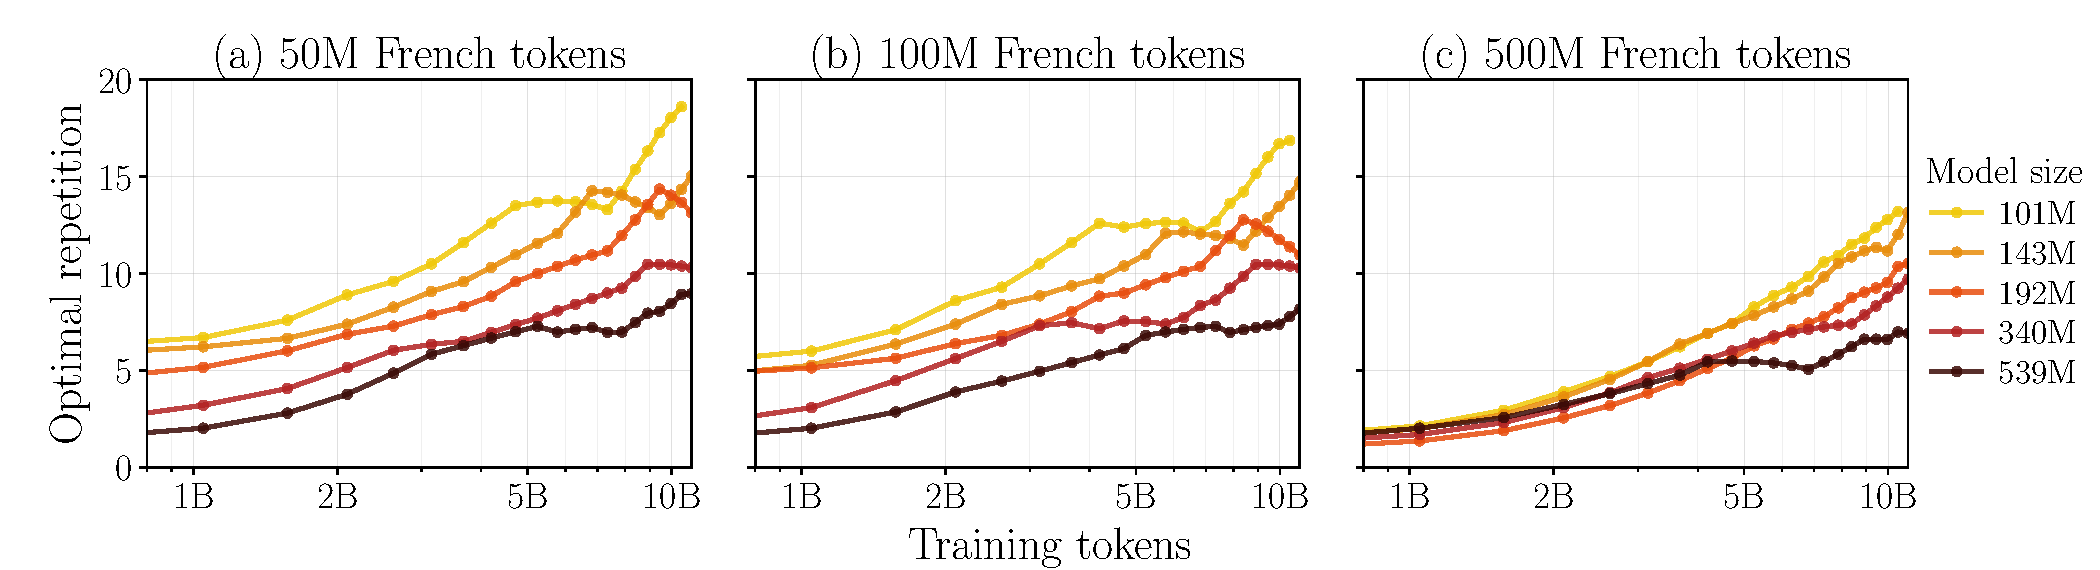
\includegraphics[width=\textwidth]{figures/appendix/fig2_optimal_r_vs_tokens_fr.pdf}
\caption{Optimal repetition as a function of training tokens for three data constraint sizes across different model sizes (French).}
\label{fig:app_optimal_r_fr}
\end{figure}
\begin{figure}[h!]
\centering
\vspace{-10pt}
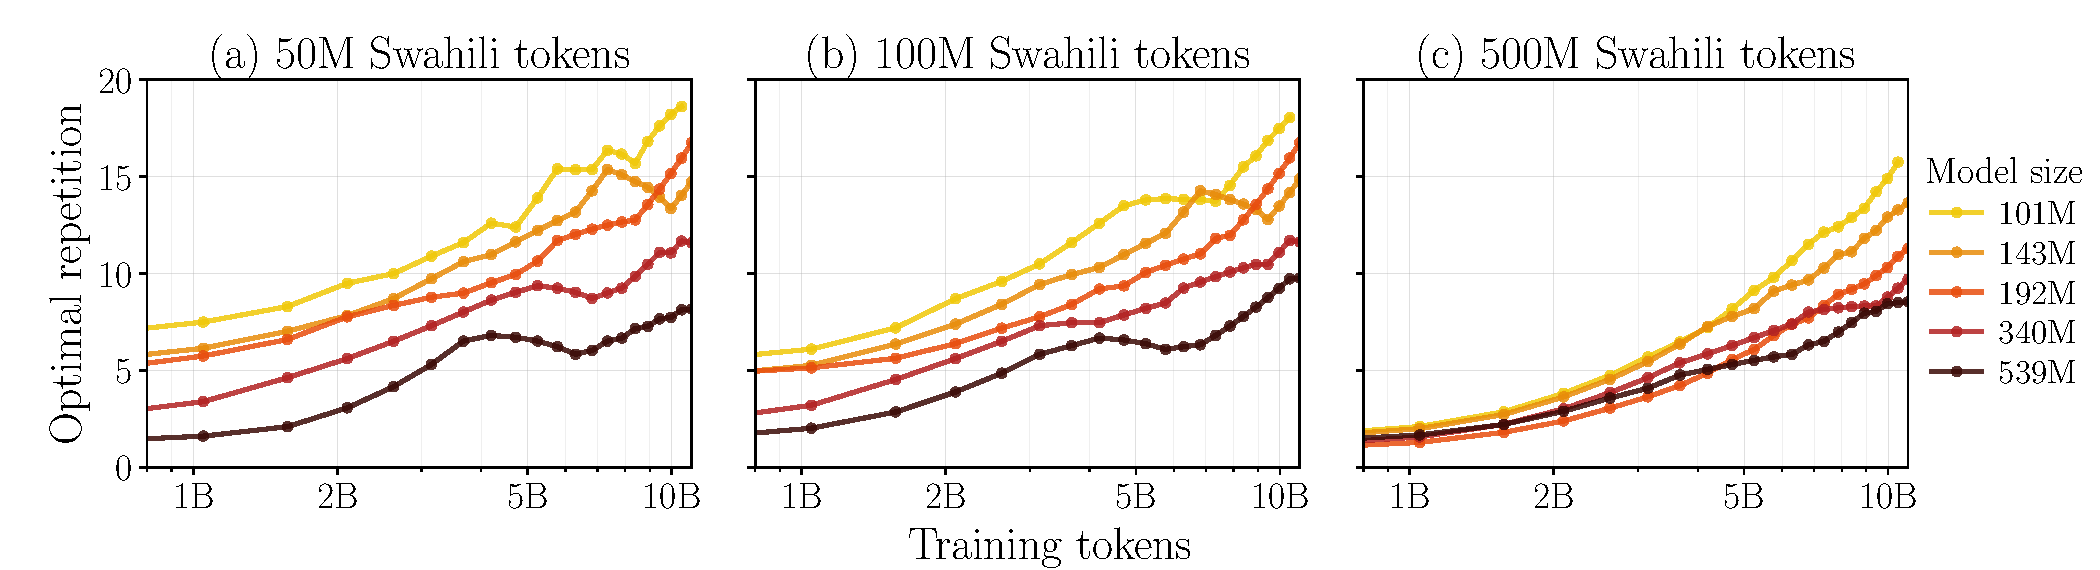
\includegraphics[width=\textwidth]{figures/appendix/fig2_optimal_r_vs_tokens_sw.pdf}
\caption{Optimal repetition as a function of training tokens for three data constraint sizes across different model sizes (Swahili).}
\label{fig:app_optimal_r_sw}
\end{figure}


Figures~\ref{fig:app_optimal_r_fr}--\ref{fig:app_optimal_r_sw} show the optimal number of repetitions as a function of training tokens for French and Swahili, matching the German plot in the main text (Figure~\ref{fig:optimal_r}). The same steady growth of optimal $r$ with training budget is observed across all languages.

\begin{figure}[h!]
\centering
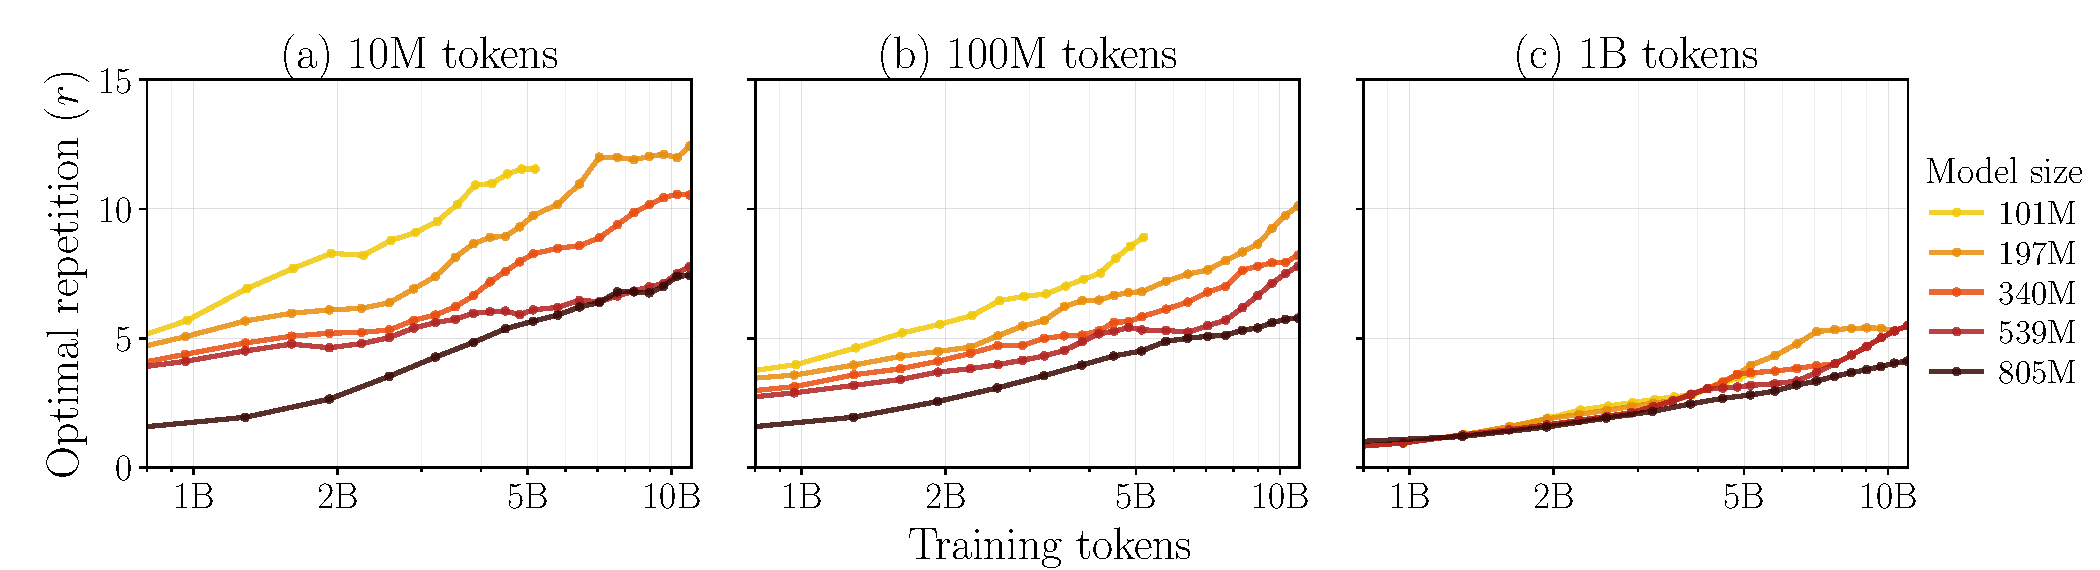
\includegraphics[width=\textwidth]{figures/appendix/fig_optimal_r_math.pdf}
\caption{Optimal repetition as a function of training tokens for three data constraint sizes across different model sizes (OpenWebMath).}
\label{fig:app_optimal_r_math}
\end{figure}


Figure~\ref{fig:app_optimal_r_math} further extends this analysis to a non-language domain: OpenWebMath mixed with DCLM as the generic source. Despite the very different nature of mathematical text, the same qualitative pattern holds: optimal $r$ increases with training tokens, decreases with pool size, and smaller models tolerate higher repetition (since they are trained on more tokens relative to their capacity). This confirms that the repetition dynamics are a general property of mixture training under data constraints, independent of the specific domain or language.

\newpage
\section{Loss Curves Across Languages, Model Sizes, and Domains}
\label{app:loss_curves}

Figures~\ref{fig:app_loss_de}--\ref{fig:app_loss_sw} show target-domain validation loss as a function of training tokens for all model sizes (101M--539M) and all three target languages (German, French, Swahili). Each column corresponds to a different target data pool size; each row to a different model size; each curve within a panel corresponds to a different target weight $h$ (color). The same qualitative pattern(i.e.,  overfitting learning curves at high $h$ with small pools, while monotonic improvement with large pools) holds consistently across all configurations.

Figure~\ref{fig:app_loss_math} shows the same analysis for OpenWebMath, confirming that the loss curve dynamics extend beyond natural language to mathematical text.

\begin{figure}[h!]
\centering
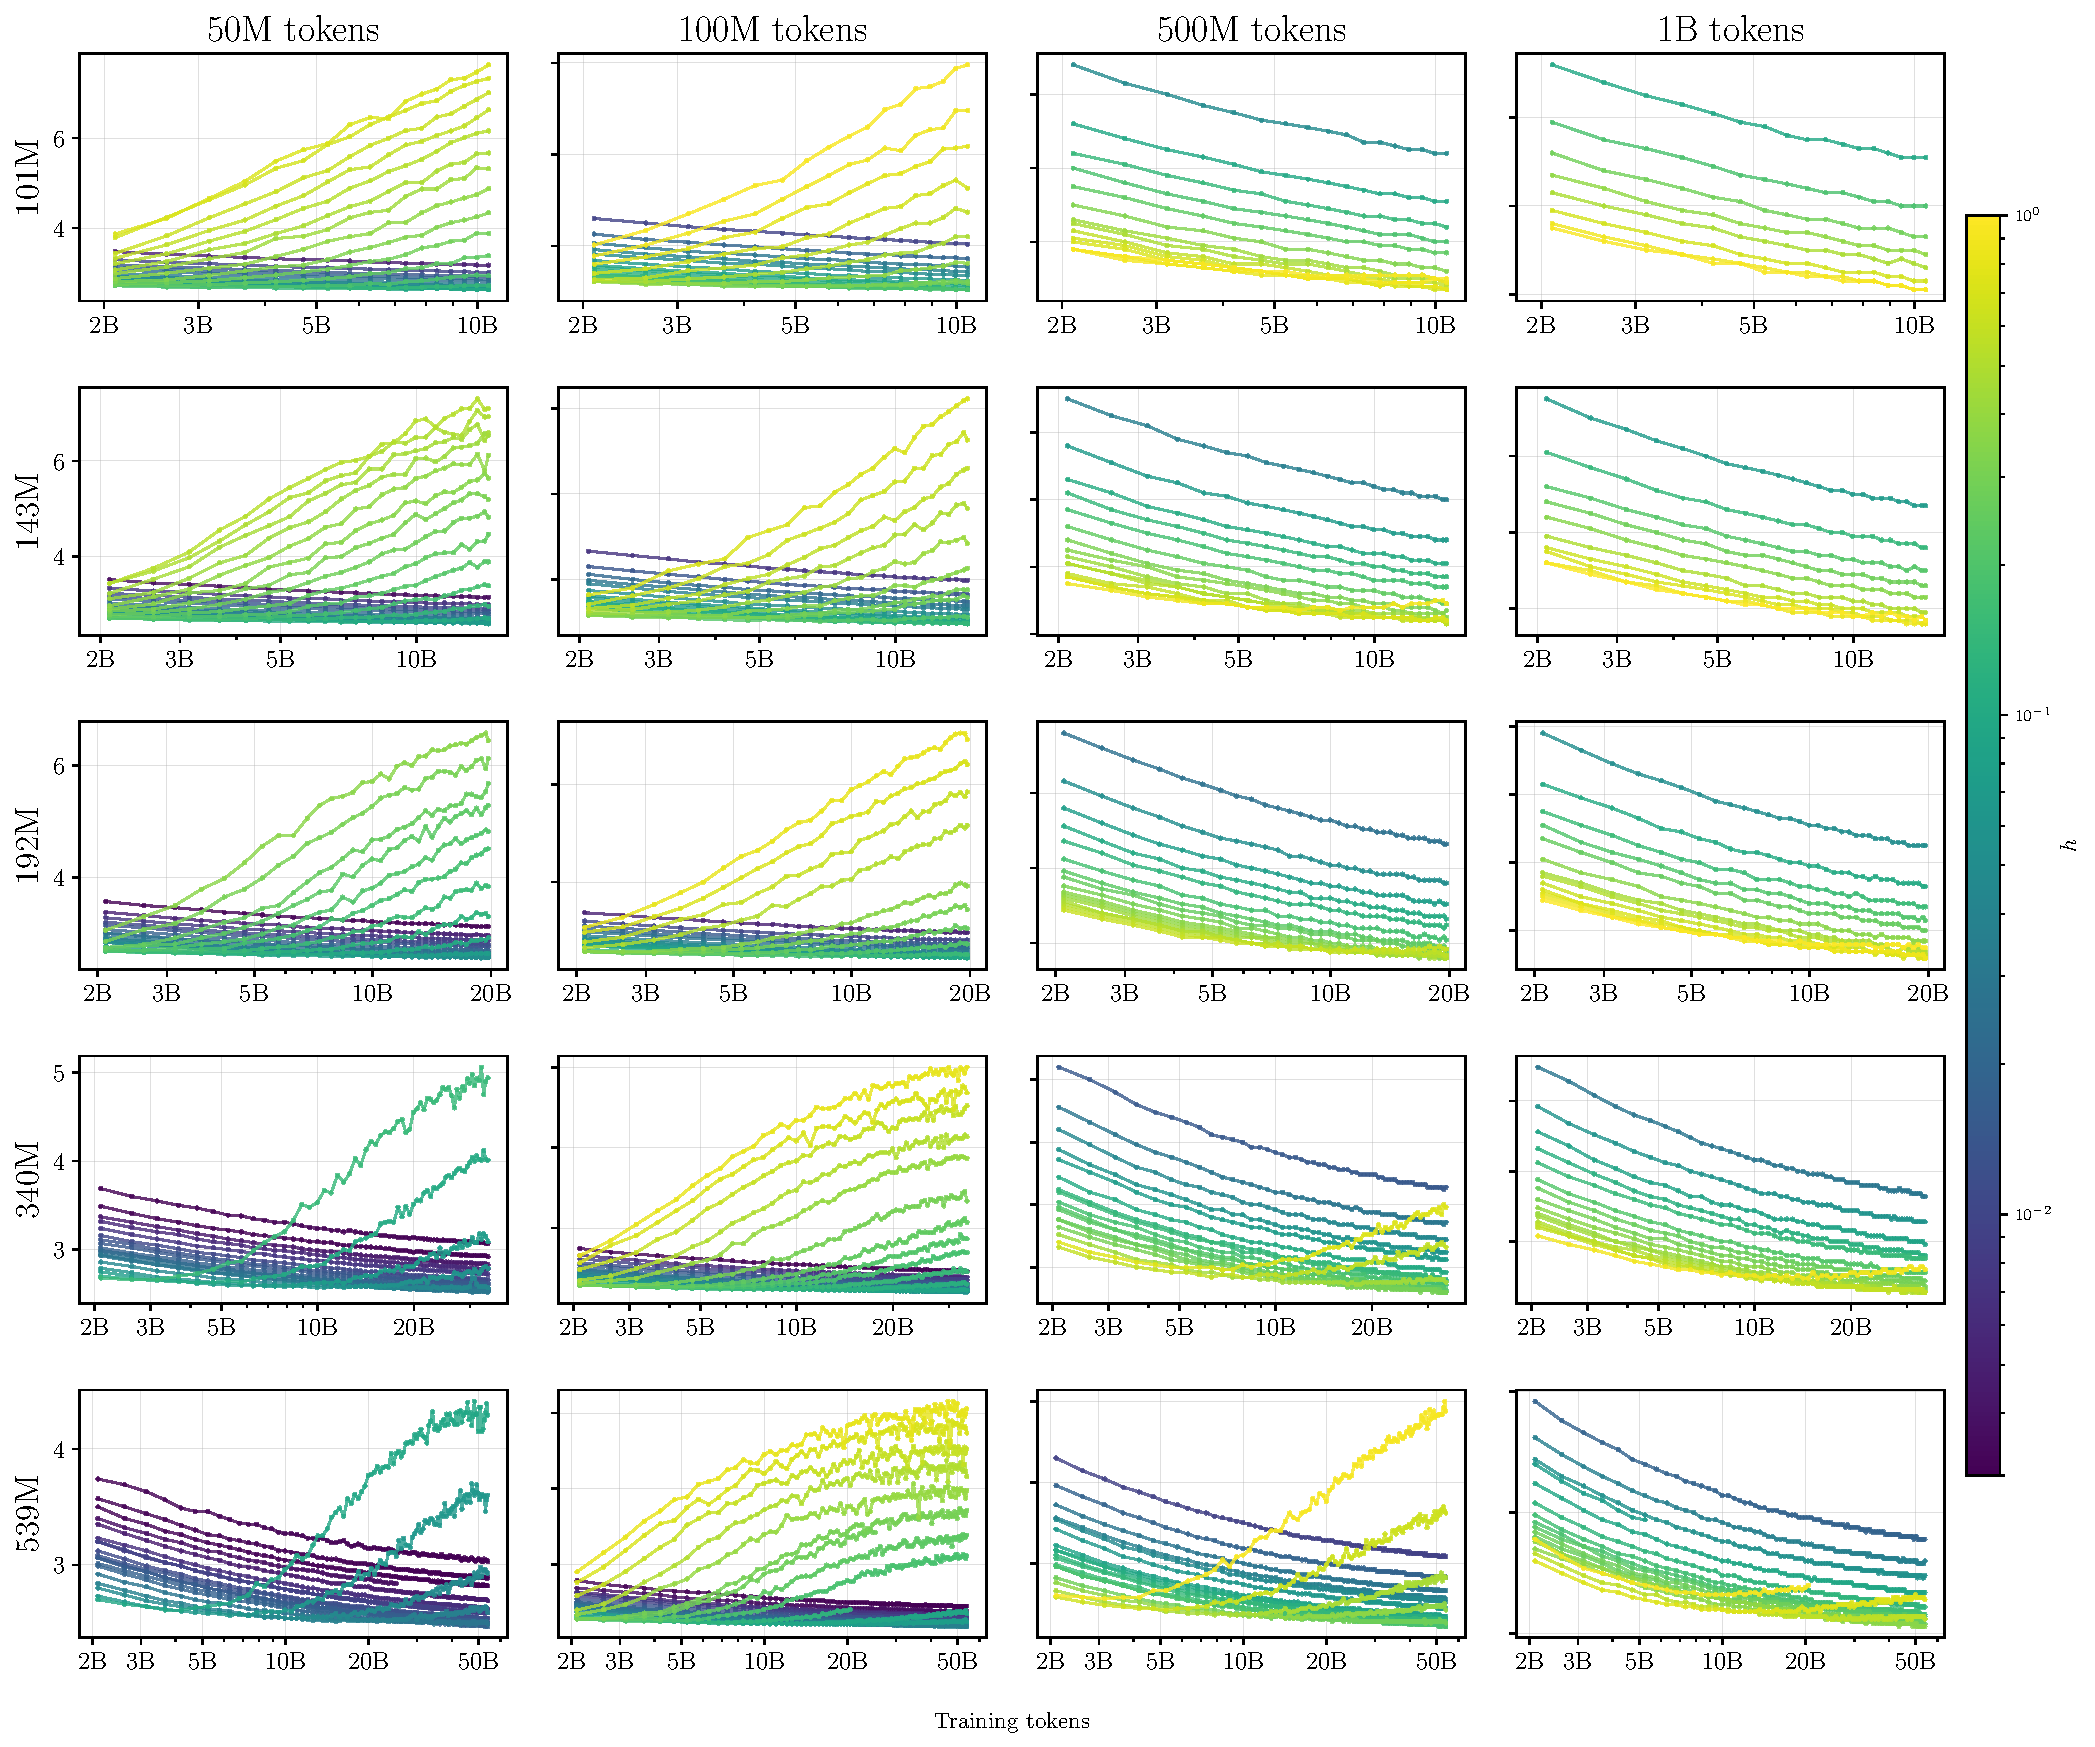
\includegraphics[width=\textwidth]{figures/appendix/loss_curves_all_de.pdf}
\caption{German target-domain loss curves across all model sizes (rows) and data pool sizes (columns).}
\label{fig:app_loss_de}
\end{figure}

\newpage
\begin{figure}[h!]
\centering
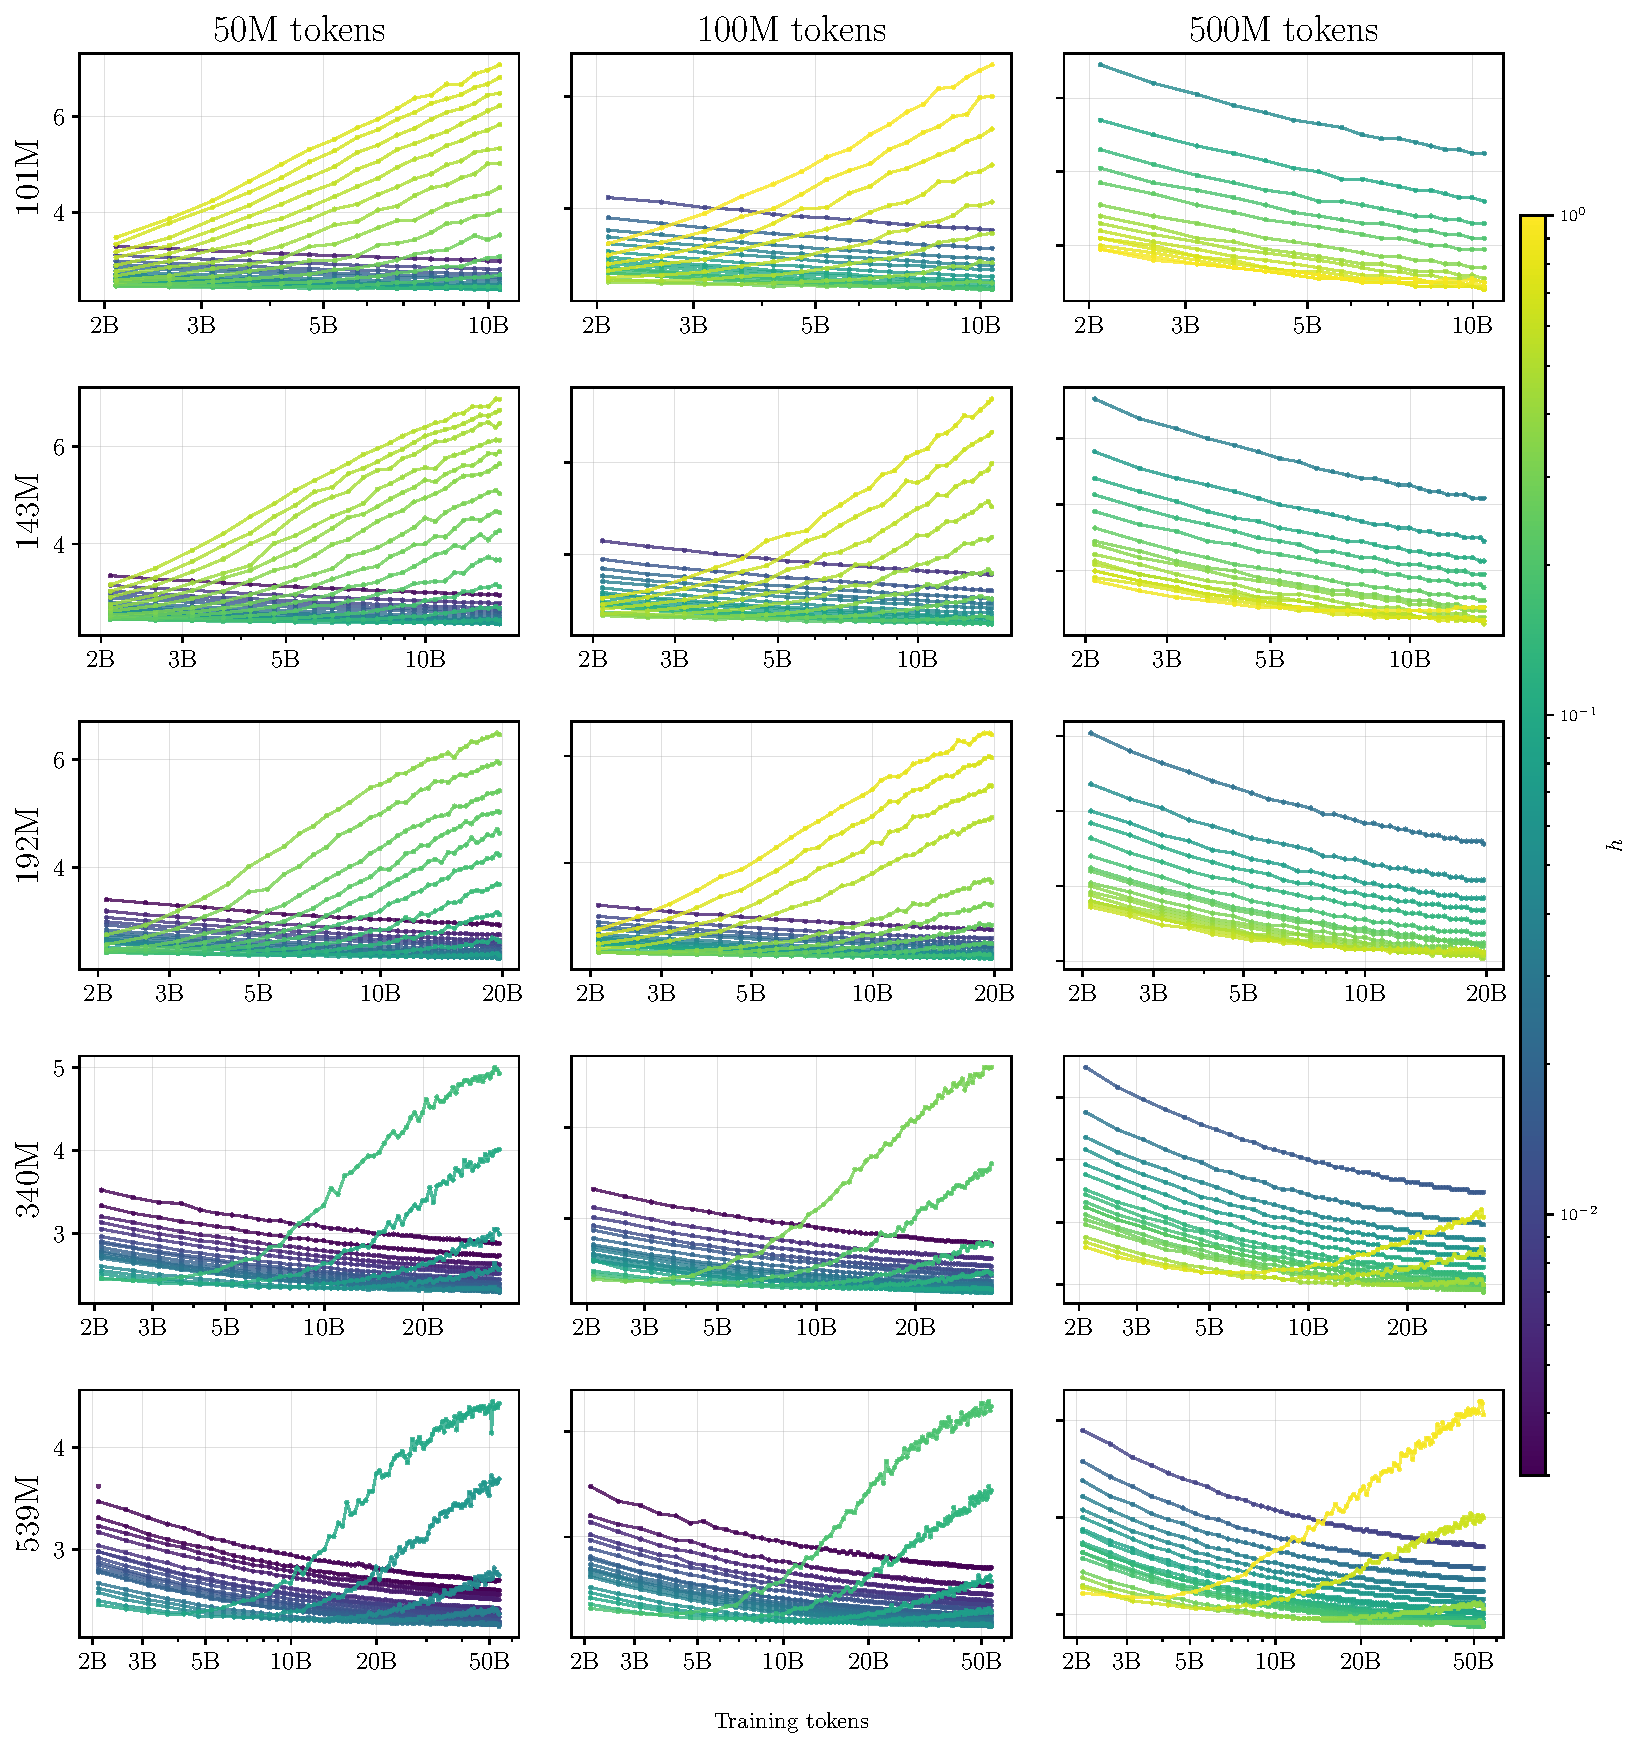
\includegraphics[width=\textwidth]{figures/appendix/loss_curves_all_fr.pdf}
\caption{French target-domain loss curves across all model sizes (rows) and data pool sizes (columns).}
\label{fig:app_loss_fr}
\end{figure}

\newpage
\begin{figure}[h!]
\centering
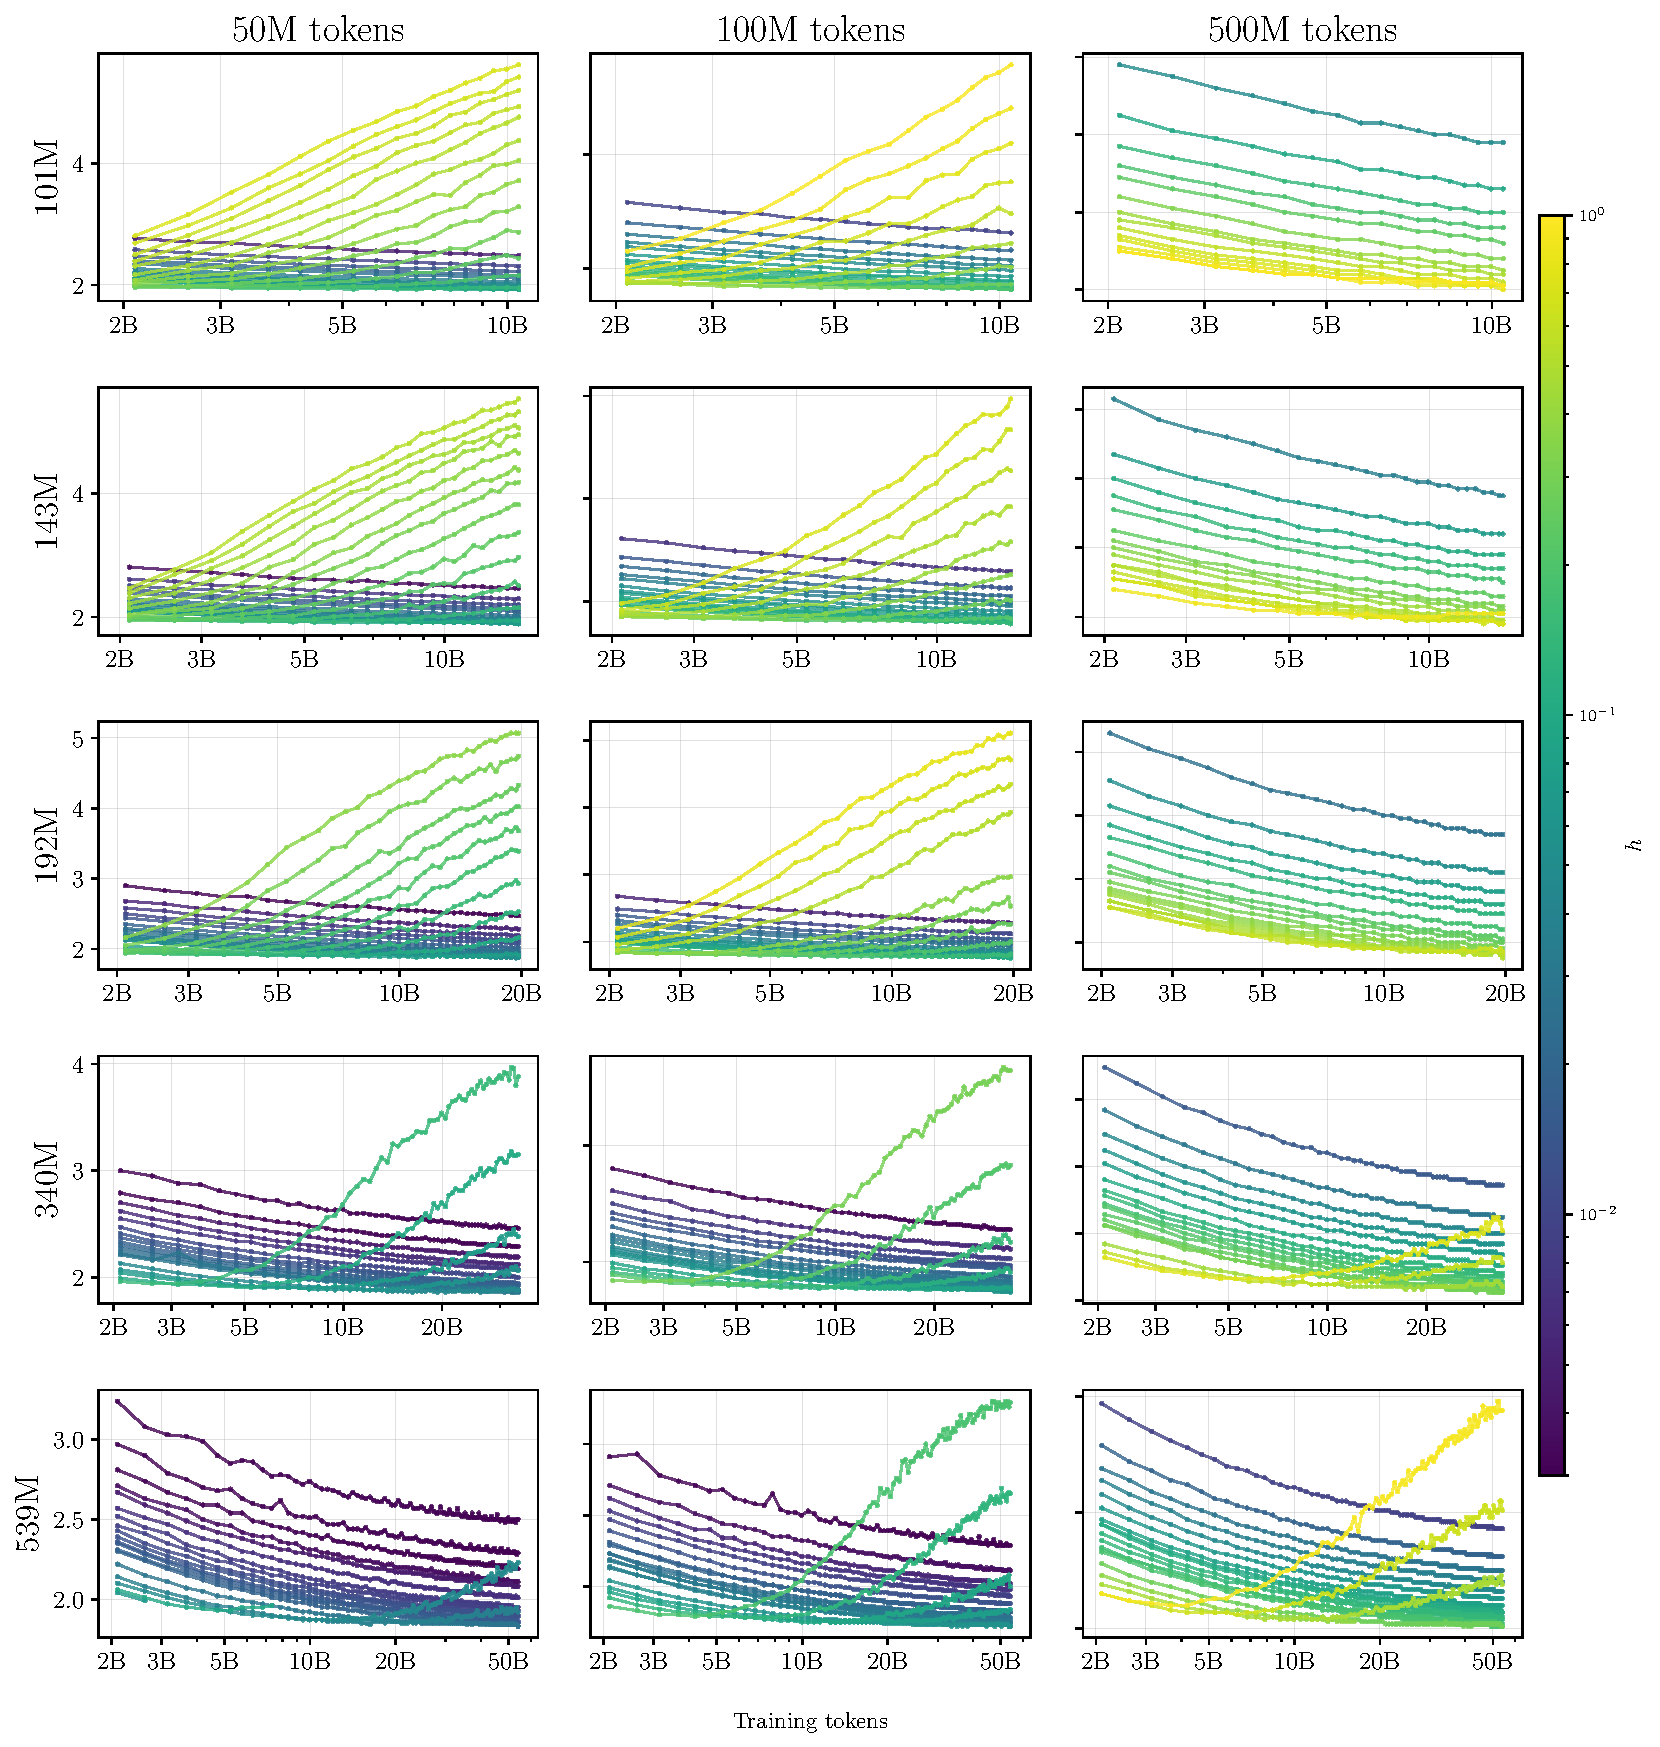
\includegraphics[width=\textwidth]{figures/appendix/loss_curves_all_sw.pdf}
\caption{Swahili target-domain loss curves across all model sizes (rows) and data pool sizes (columns).}
\label{fig:app_loss_sw}
\end{figure}

\newpage
\begin{figure}[h!]
\centering
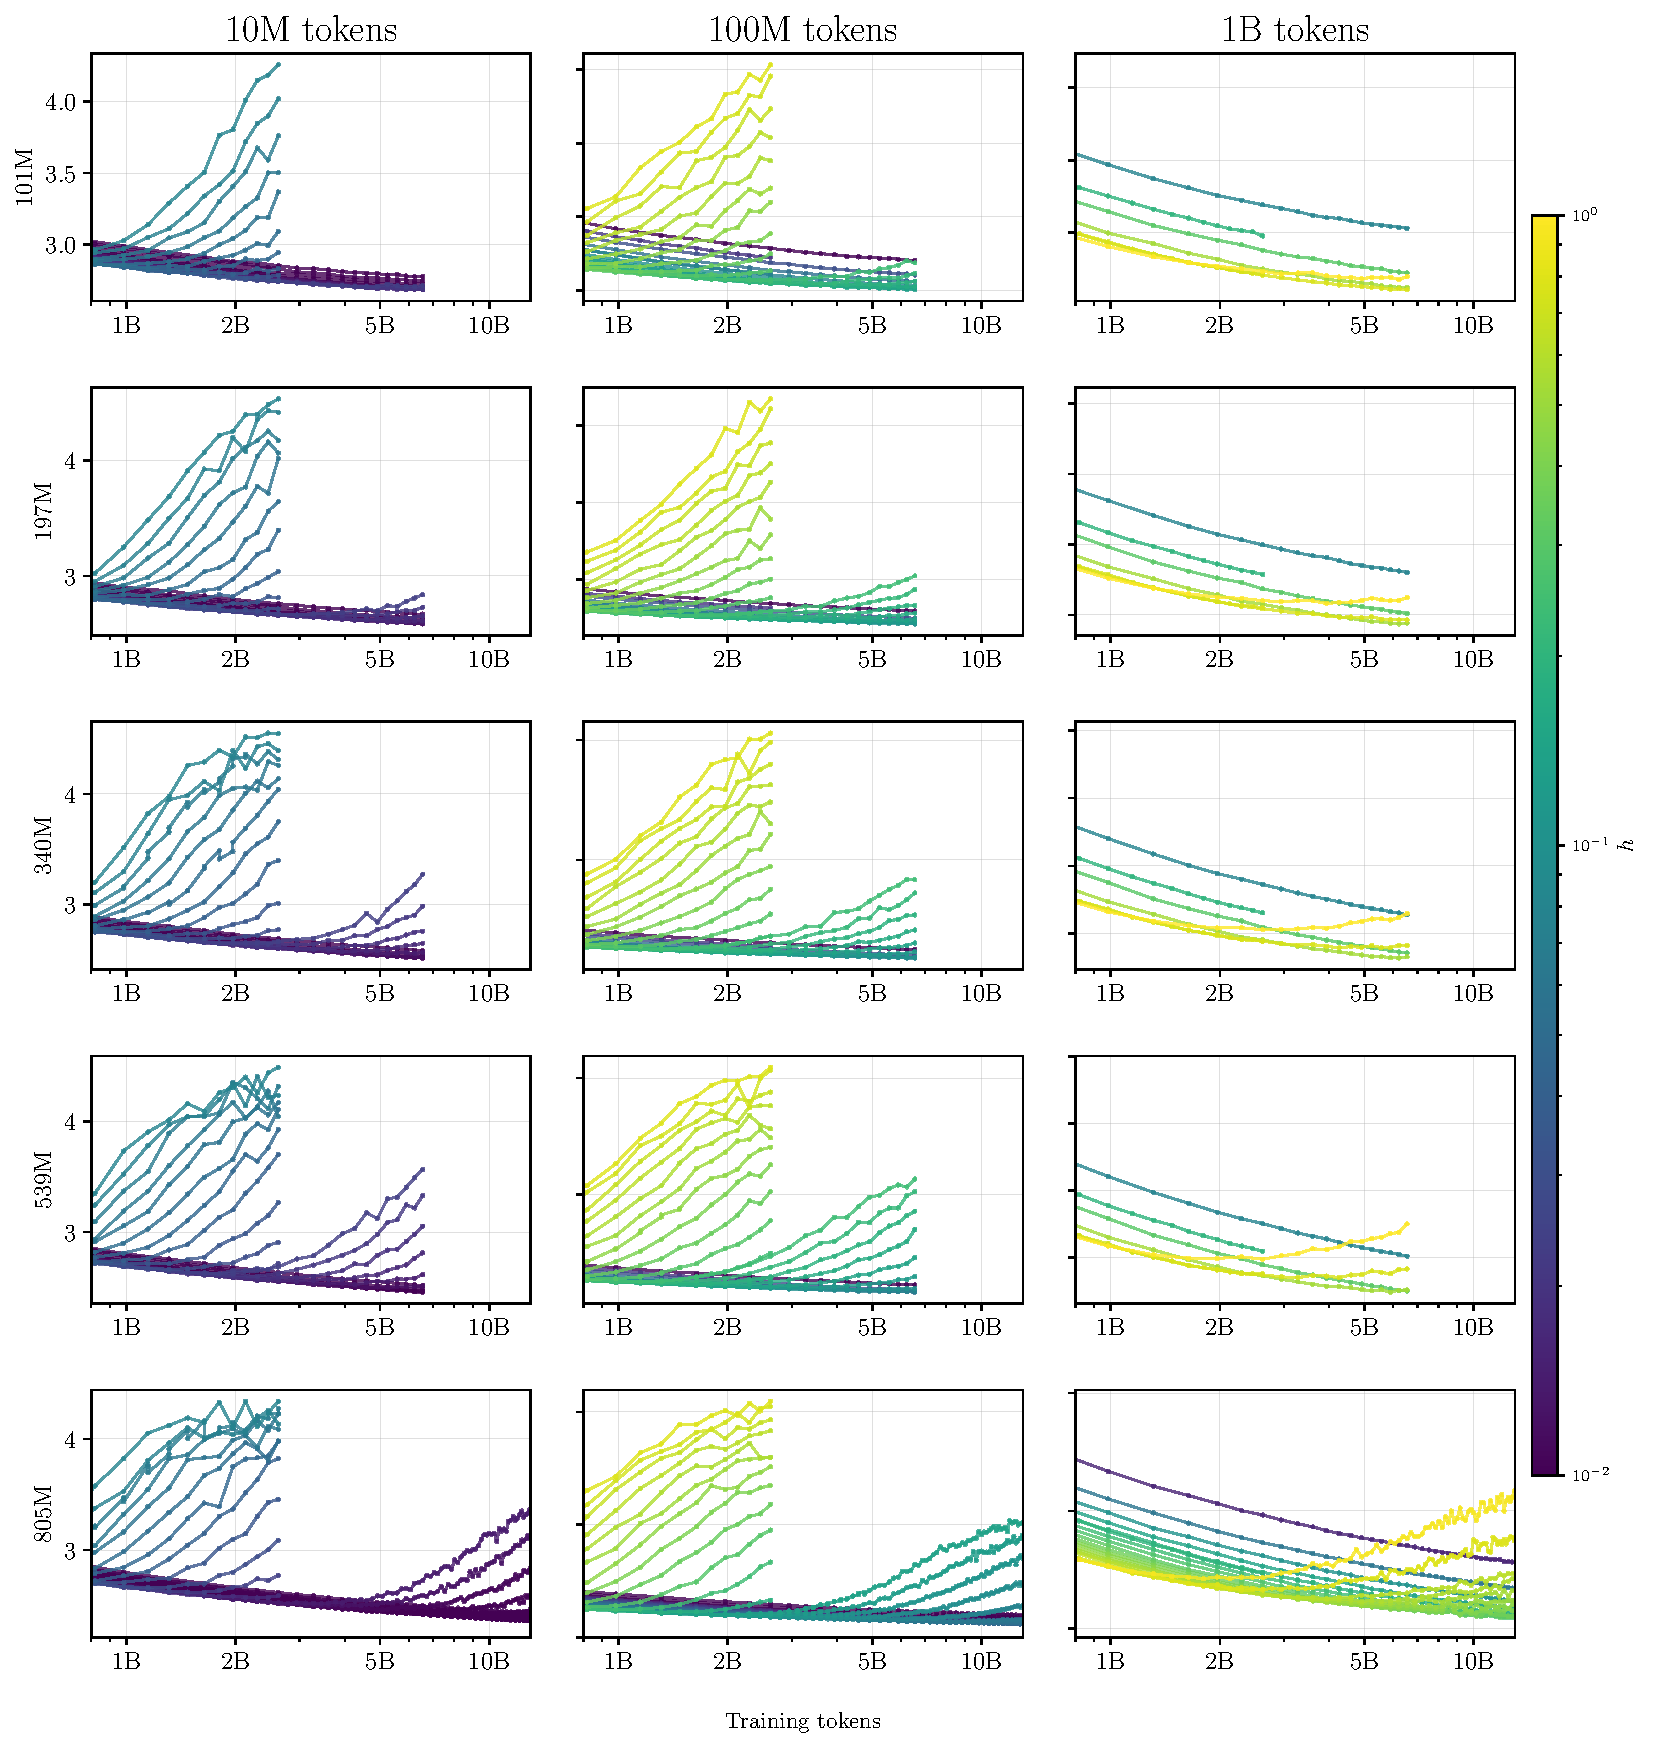
\includegraphics[width=\textwidth]{figures/appendix/loss_curves_all_math.pdf}
\caption{Math (OpenWebMath) target-domain loss curves across all model sizes (rows) and data pool sizes (columns).}
\label{fig:app_loss_math}
\end{figure}



\newpage
\section{Cross-Model Loss Curves}
\label{app:cross_model}

Figure~\ref{fig:cross_model_fixed_h} shows that larger models overfit faster yet achieve lower best-case loss, demonstrated for German with 100M tokens at $h = 9\%$ and $20\%$. Here we extend this analysis to five target fractions (5--20\%) and verify the pattern across all languages and domains. Figure~\ref{fig:cross_model_de} shows the full German panel, Figures~\ref{fig:cross_model_fr}--\ref{fig:cross_model_sw} show French and Swahili, and Figure~\ref{fig:math_cross_model} shows the OpenWebMath domain. In all cases, the same ordering persists: larger models reach lower loss minima despite earlier overfitting onset, and the best-loss envelope (dashed) consistently favors larger models at every training budget. The pattern is particularly pronounced for the mathematics domain (Figure~\ref{fig:math_cross_model}), where the separation between model sizes is larger and the overfitting onset for larger models is sharper.

\begin{figure}[h!]
\centering
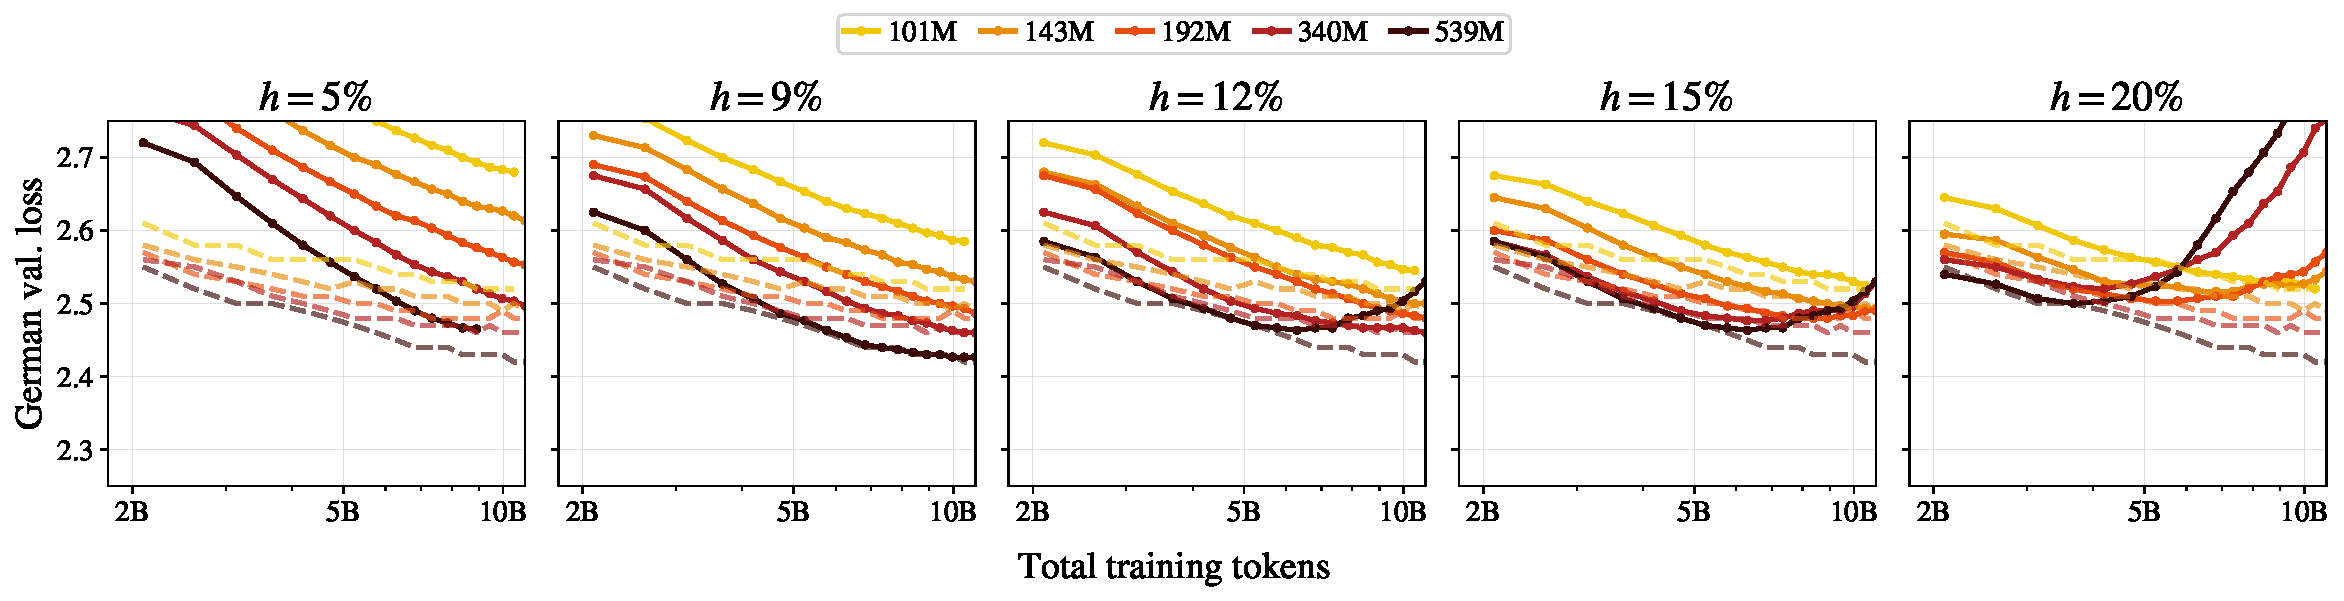
\includegraphics[width=\textwidth]{figures/loss_curves_by_weight_de_100M_5panel.pdf}
\caption{German target-domain loss across model sizes at five target fractions, for the 100M token pool. Dashed lines show the best-loss envelope.}
\label{fig:cross_model_de}
\end{figure}

\begin{figure}[h!]
\centering
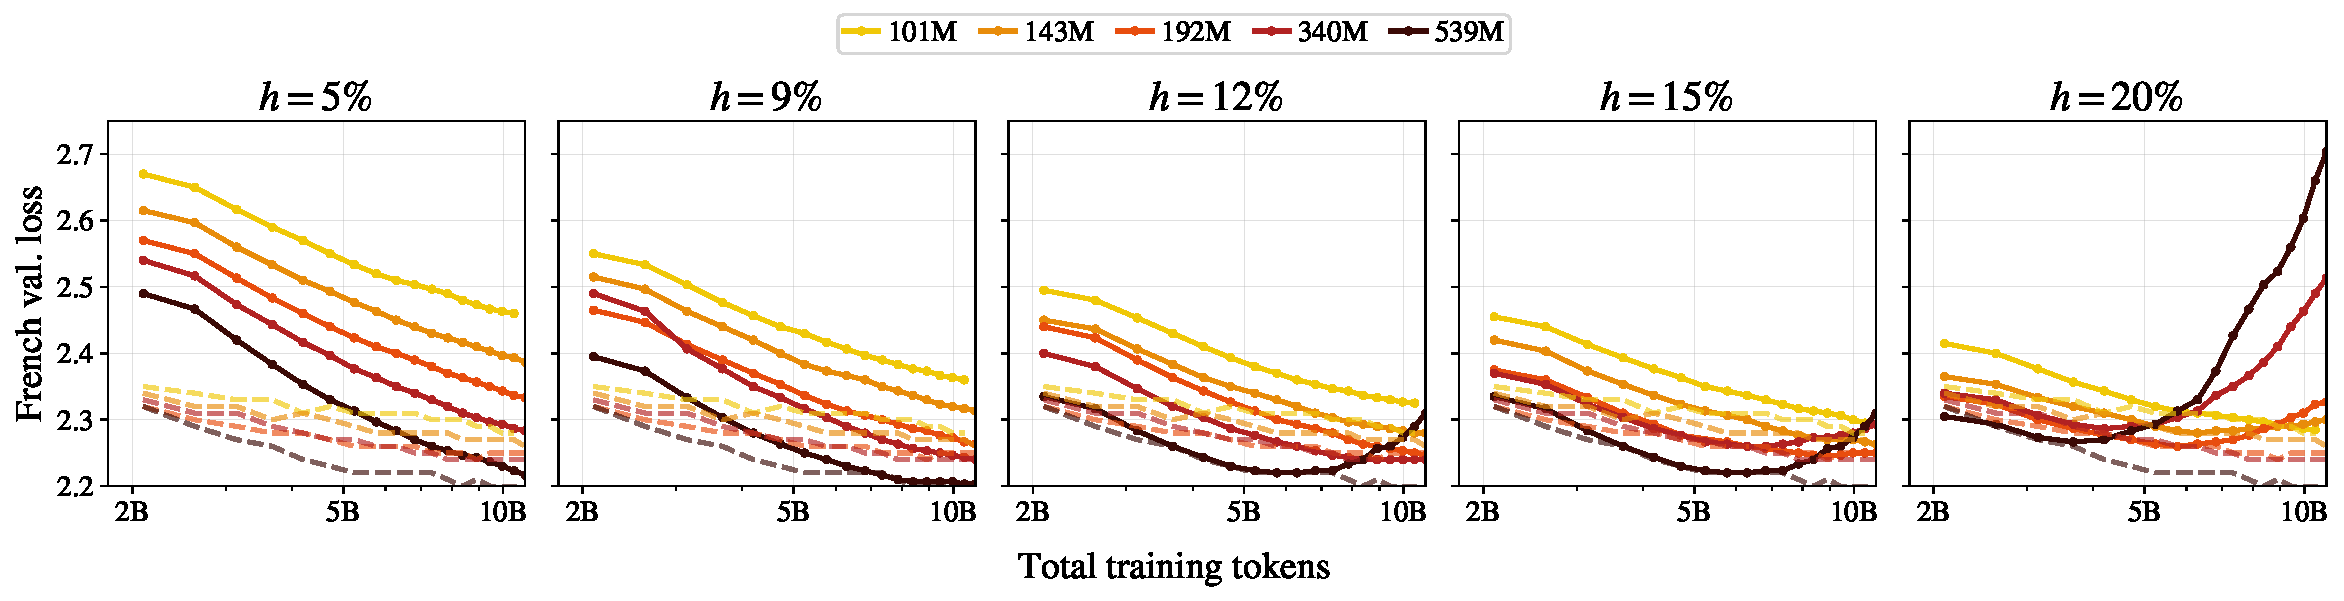
\includegraphics[width=\textwidth]{figures/loss_curves_by_weight_fr_100M_5panel.pdf}
\caption{French target-domain loss across model sizes at five target fractions, for the 100M token pool. Dashed lines show the best-loss envelope.}
\label{fig:cross_model_fr}
\end{figure}

\begin{figure}[h!]
\centering
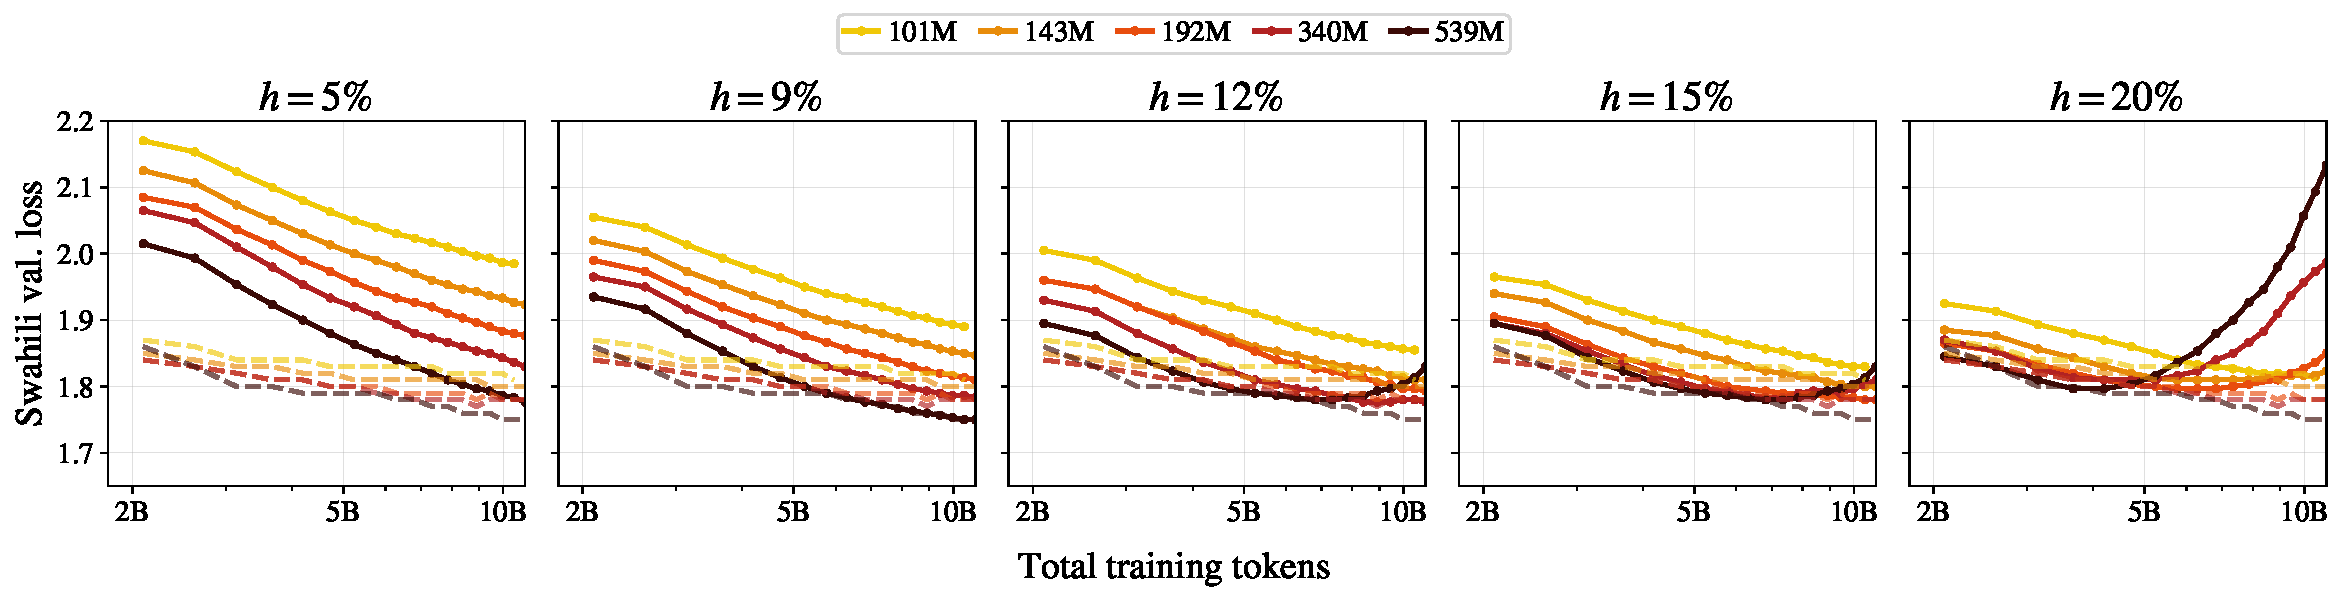
\includegraphics[width=\textwidth]{figures/loss_curves_by_weight_sw_100M_5panel.pdf}
\caption{Swahili target-domain loss across model sizes at five target fractions, for the 100M token pool. Dashed lines show the best-loss envelope.}
\label{fig:cross_model_sw}
\end{figure}

\begin{figure}[h!]
\centering
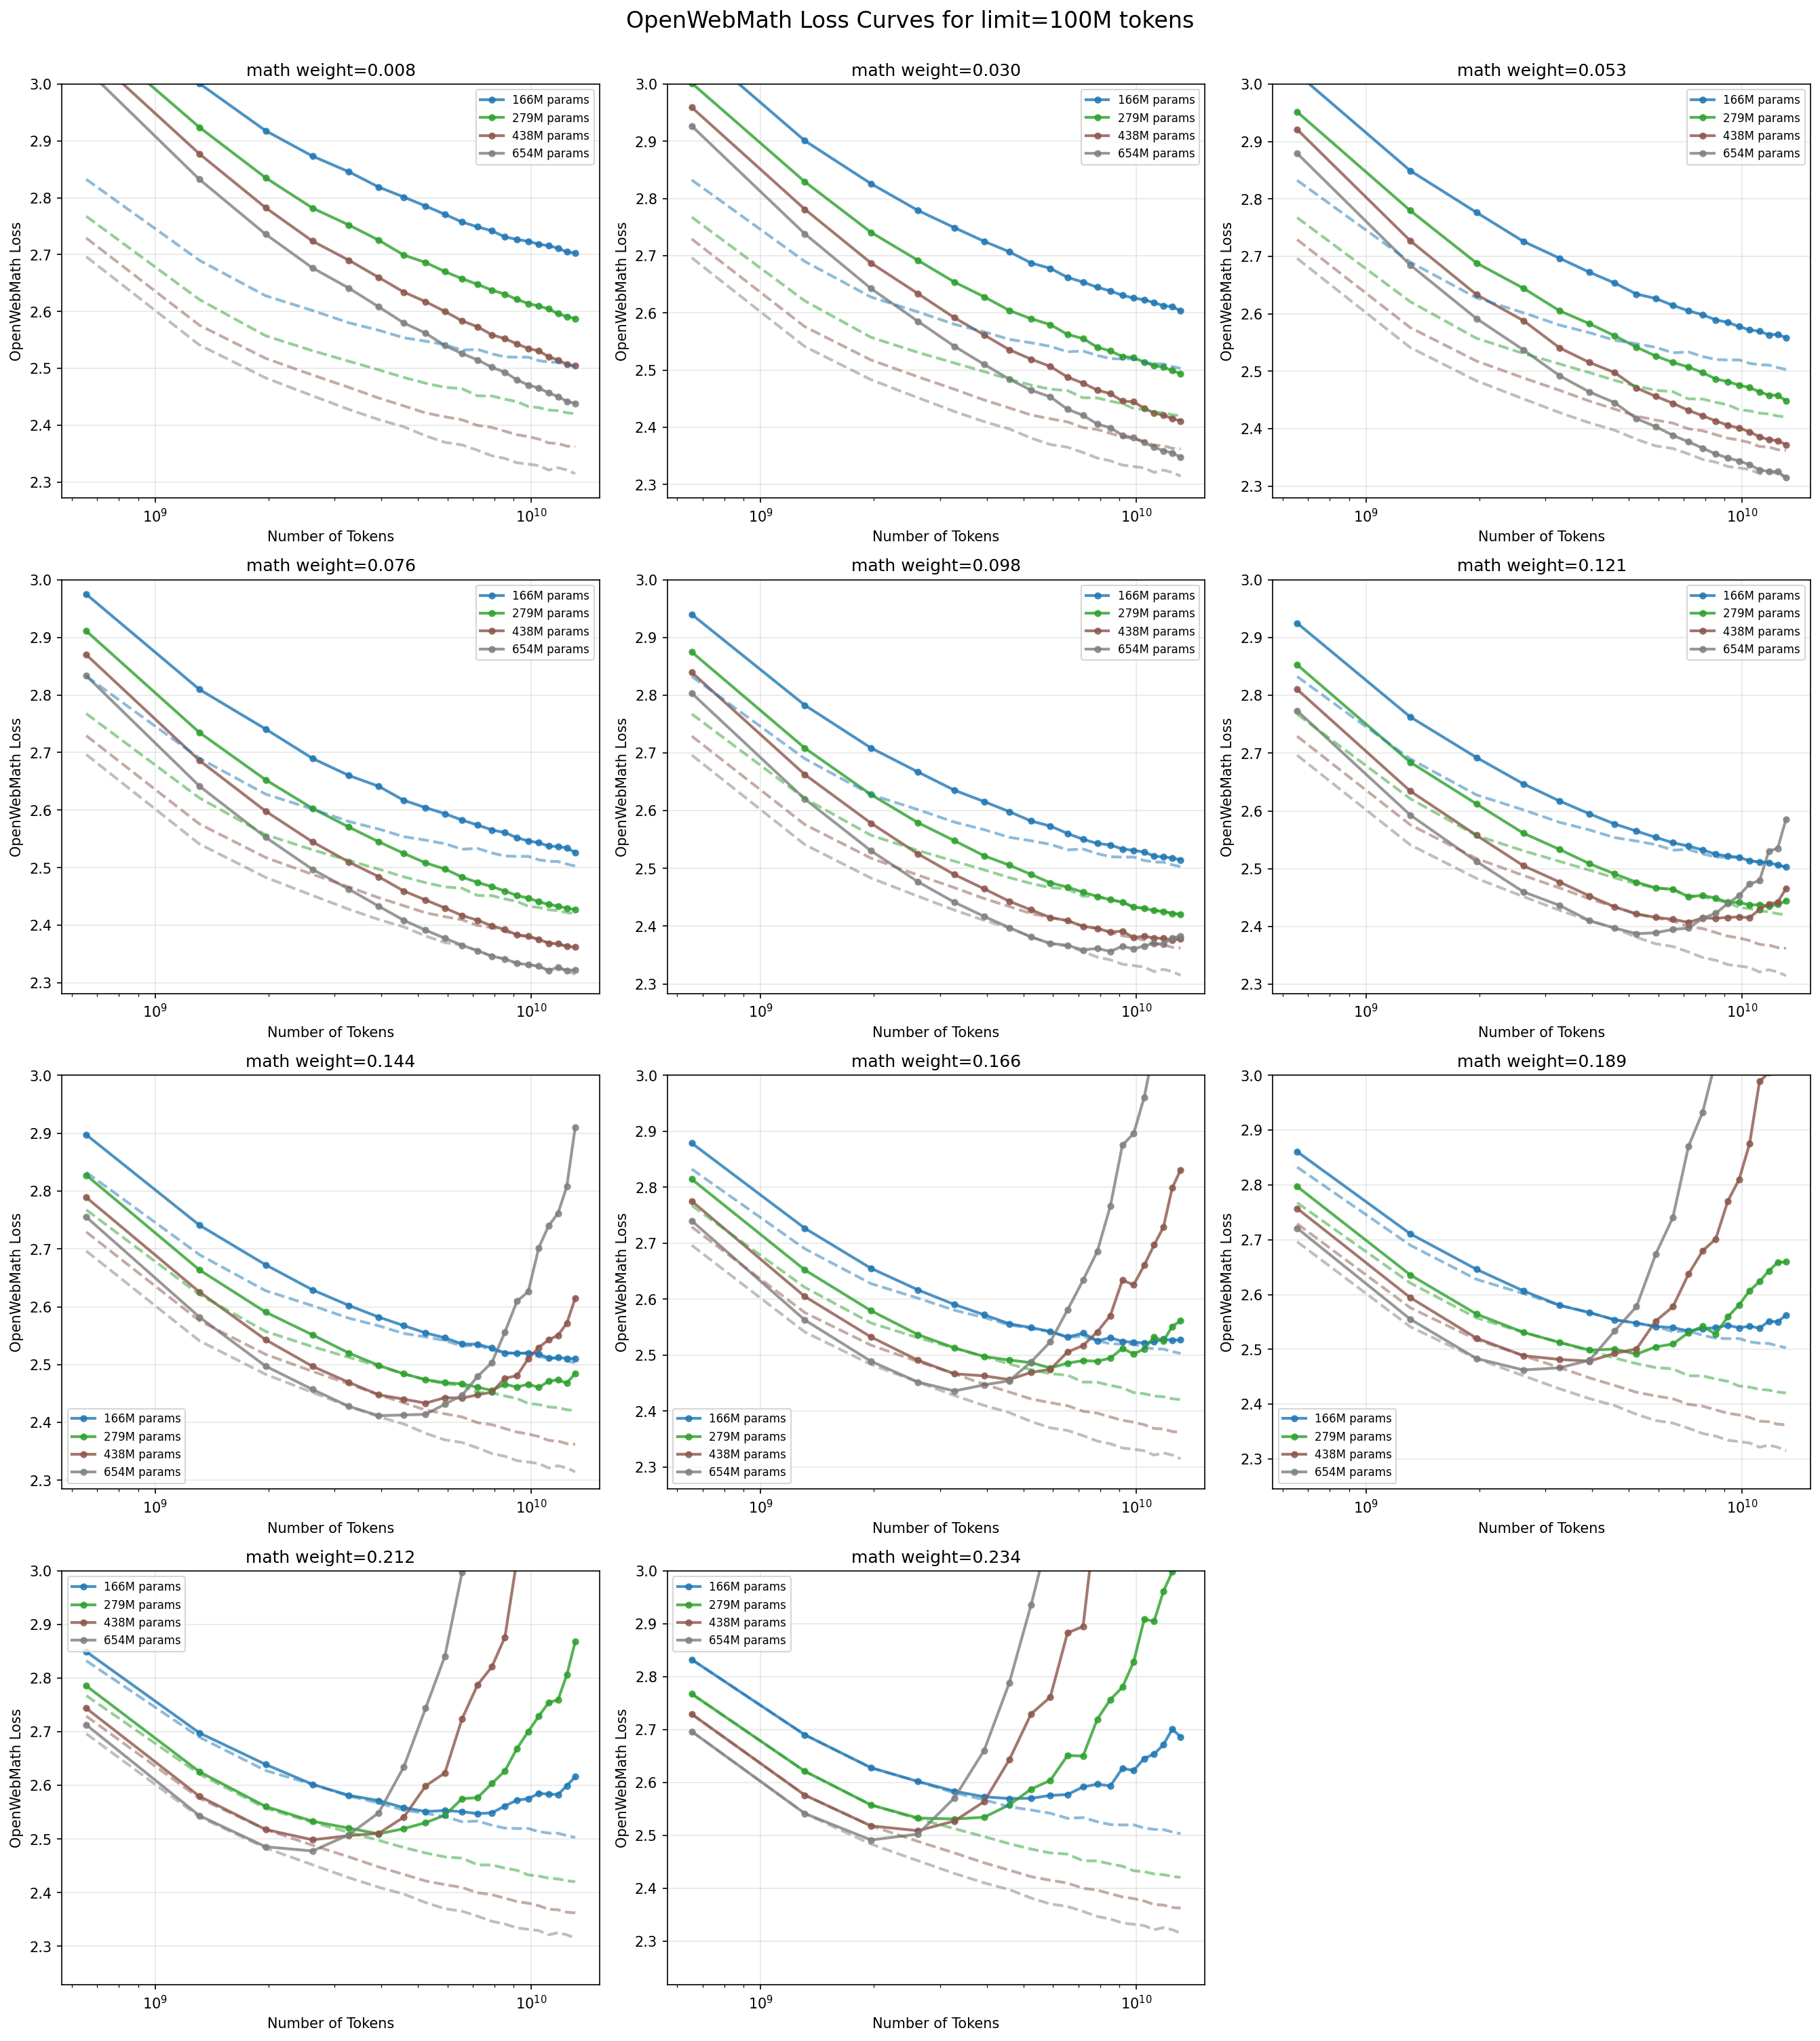
\includegraphics[width=\textwidth]{figures/loss_curves_by_weight_math_100M.png}
\caption{OpenWebMath target loss across model sizes at different mixture fractions $h$, for the 100M token pool. Dashed lines show the best-loss envelope across all $h$ values.}
\label{fig:math_cross_model}
\end{figure}


\newpage
\section{Quality Experiments: Additional Target Data Scales and Overlapping Quality Pools}
\label{app:quality_scales}

To ground the experiments, we first confirm that a data constrained fixed quality level follows the same pattern as multilingual data. Figure~\ref{fig:top_1_data_constrained} shows Q99--100 loss curves at three pool sizes (26M, 132M, 264M tokens). At the smallest scale, only $h \leq 0.1$ avoids overfitting, and larger pools progressively unlock higher sustainable target weights.
This establishes the baseline that for a fixed quality threshold, the repetition penalty imposes the same constraint on the target loss.

\begin{figure}[h!]
    \centering
    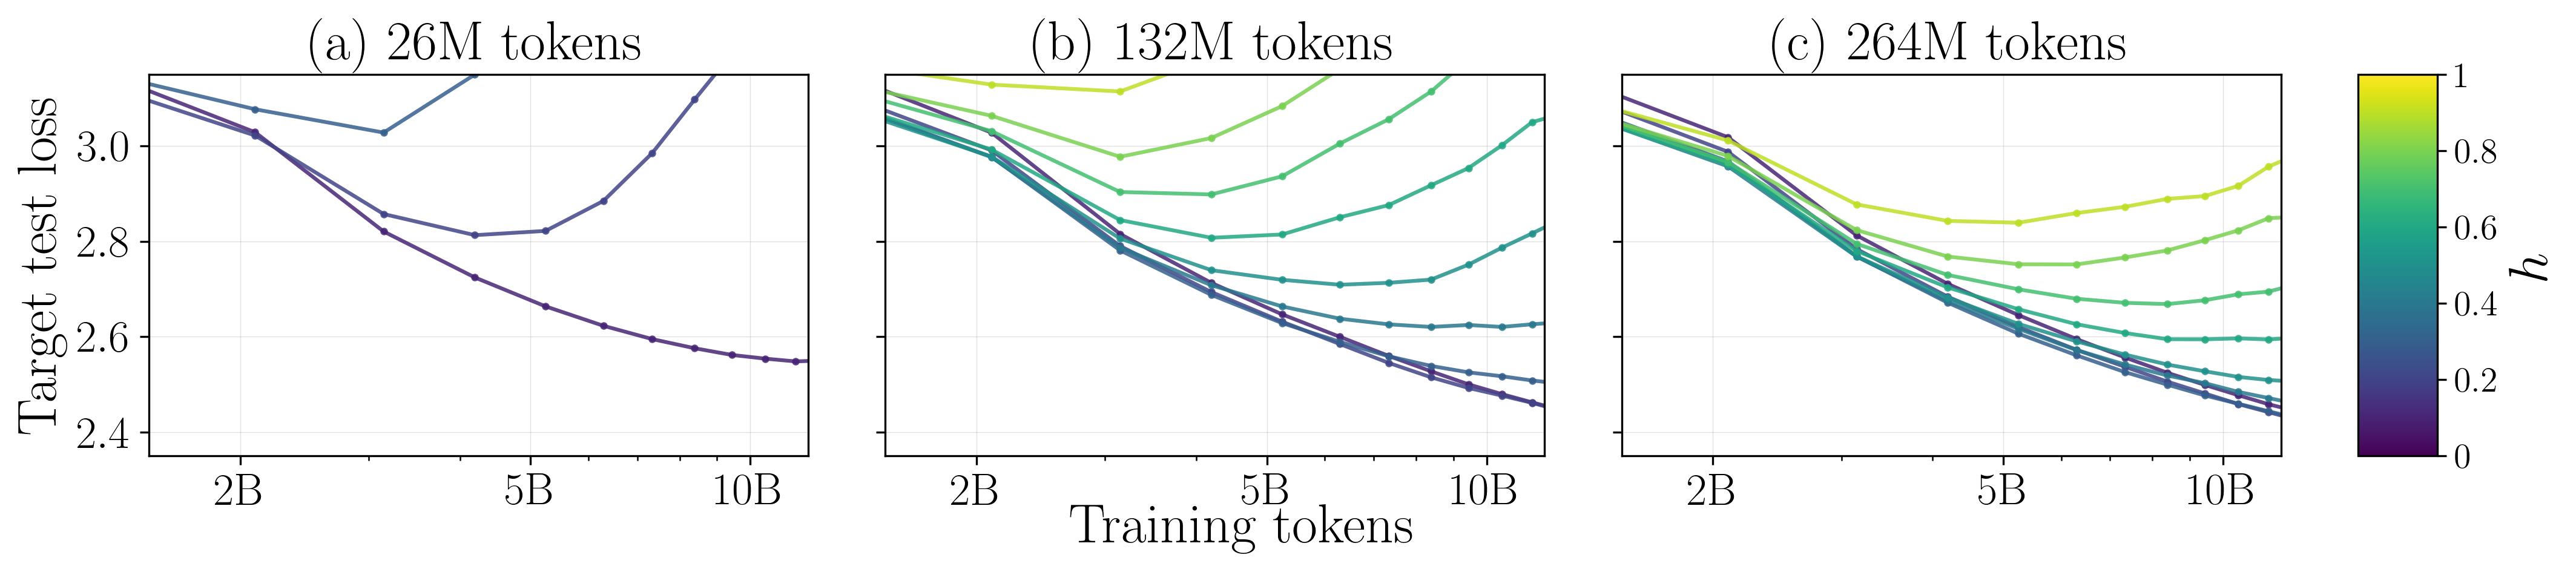
\includegraphics[width=\textwidth]{figures/paper_quality_data_constrained.png}
    \caption{Loss vs. training tokens for Q99--100 at three data pool sizes. Each line corresponds to a target weight $h$. Smaller pools force lower weights to avoid overfitting from repetition.}
    \label{fig:top_1_data_constrained}
\end{figure}

\Cref{sec:results} further establishes that when training with a data-constrained high-quality domain, relaxing the quality filter to increase pool size consistently outperforms repeating the highest-quality slice starting from the 26M 99th percentile data pool.
A crossover at 5B tokens shows the optimal threshold shifts from Q95--99 to Q90--99 as training progresses. Here we present an expanded experimental suite, including additional data scales that support and extend these findings. We conduct three families of experiments, all using 100M-parameter models trained on a two-domain mixture of high-quality (HQ) filtered text and unlimited general DCLM. Each experiment sweeps target weight $w \in \{0.1, 0.2, \ldots, 1.0\}$.

\paragraph{Non-overlapping quality buckets at multiple data scales}
We define non-overlapping quality bands (Q90--99, Q95--99, Q99--100) and train at three data scales:
\begin{itemize}[nosep]
    \item \textbf{1$\times$}: pools range from 26M to 982M tokens including severe data constraint, and high repetition especially for high quality data.
    \item \textbf{5$\times$}: pools range from 132M to 2.1B tokens. This imposes a moderate constraint where the highest qualitybuckets have high repetition counts, but lower quality buckets do not.
    \item \textbf{10$\times$}: pools range from 264M to 4.2B tokens. Most quality buckets avoid significant repetition, and only the highest quality bucket still overfits with too much repetition.
\end{itemize}

\begin{figure}[h!]
  \centering
  \begin{subfigure}[t]{\textwidth}
      \centering
      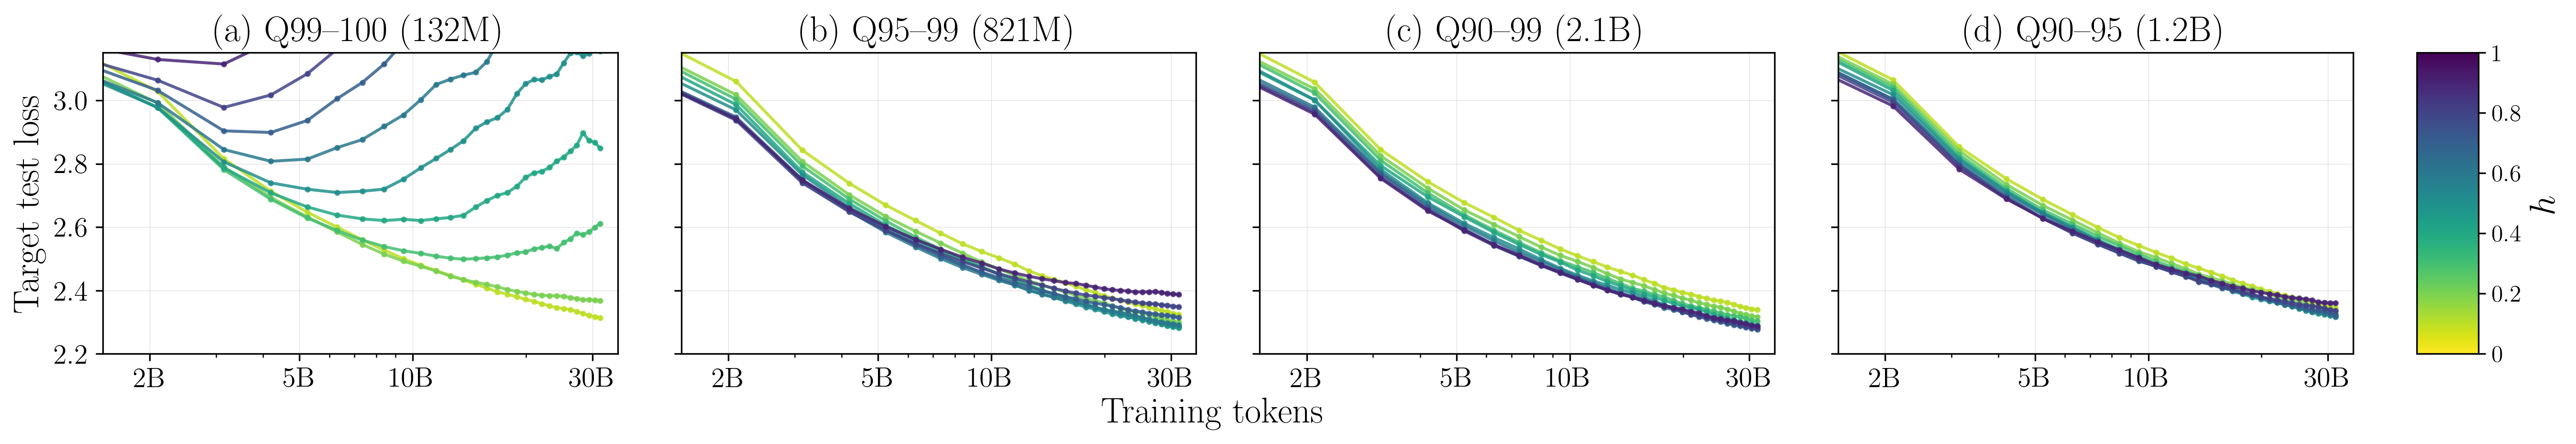
\includegraphics[width=\textwidth]{figures/paper_comparison_1x_combined.png}
      \caption{Pool sizes: Q99–100 (132M), Q95–99 (821M), Q90–99 (2.1B), Q90–95 (1.2B).}
      \label{fig:quality_1x}
  \end{subfigure}


  \begin{subfigure}[t]{\textwidth}
      \centering
      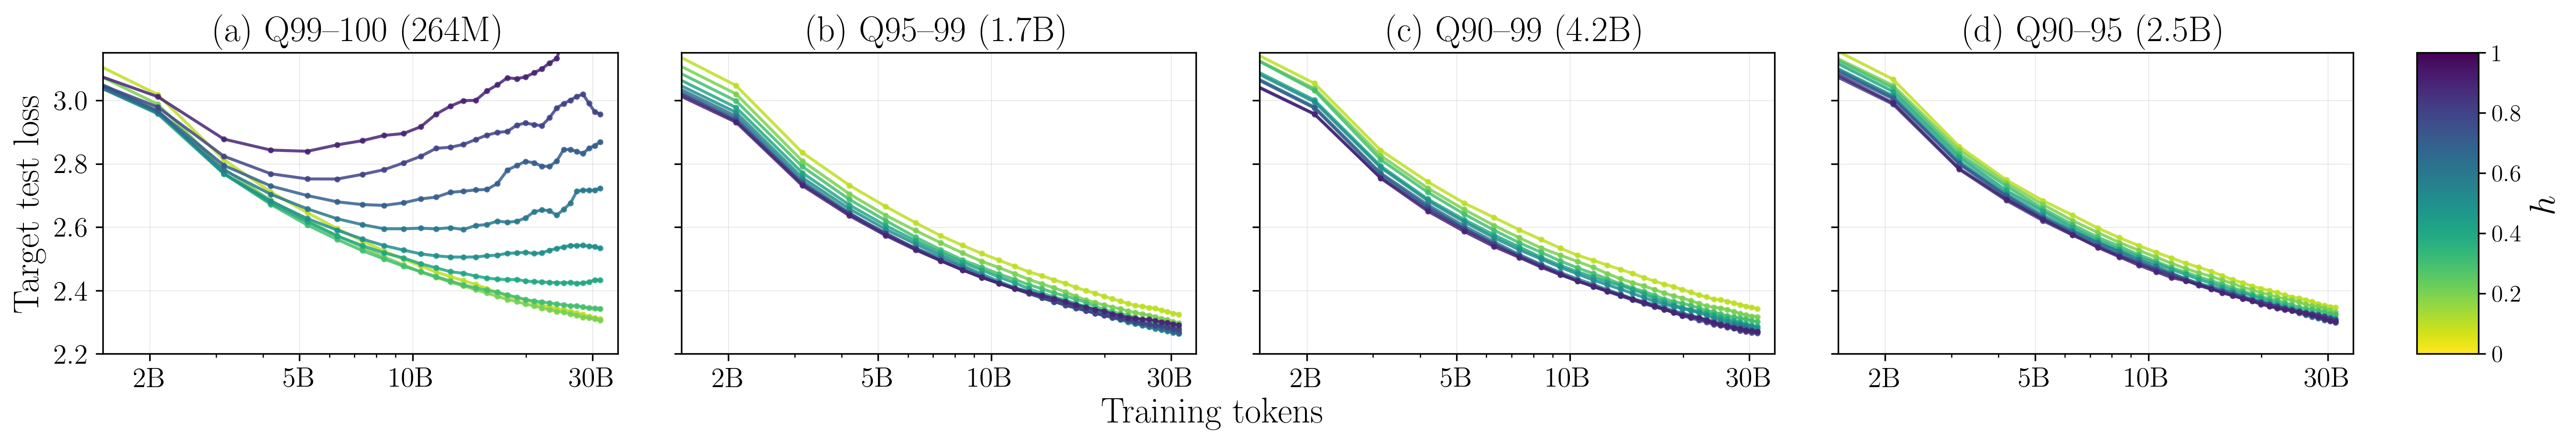
\includegraphics[width=\textwidth]{figures/paper_comparison_2x_combined.png}
      \caption{Pool sizes: Q99–100 (264M), Q95–99 (1.7B), Q90–99 (4.2B), Q90–95 (2.5B).}
      \label{fig:quality_2x}
  \end{subfigure}

  \caption{Loss curves for four quality bands at increasing data scales. Each line corresponds to a mixture weight $h$. Broader quality filters enable higher mixture weights without overfitting, with the effect diminishing as pool size increases.}
  \label{fig:quality_1x_2x}
  \end{figure}

These experiments disentangle quality from quantity by ensuring no data overlap between bands, and reveal how the quality--quantity tradeoff evolves with different data constrained data scales.  Scaling up from the 26M target data pool to 5$\times$ and 10$\times$ the pool size confirms the main findings and reveals how the quality--quantity tradeoff evolves with data availability. At 5$\times$, Q95--99 dominates for the first ${\sim}$14B tokens before Q90--99 overtakes it (\Cref{fig:quality_1x}). The same crossover is observed at 1$\times$ but shifted later due to the larger pool delaying saturation. At 10$\times$, Q95--99 remains the best band throughout 30B tokens of training (\Cref{fig:quality_2x}): with data pools exceeding 1.6B tokens, no band experiences meaningful repetition at reasonable values of $h$, and higher per-token quality is the dominant factor. This demonstrates that the quality--quantity tradeoff is scale-dependent: at small scales, breadth wins; at large scales, quality wins; and the crossover token count increases predictably with pool size.  We include results with Q90-95 as a control to show that simply increasing the amount of data but decreasing quality performs worse.  The best-loss per quality over all $h$ is shown in \Cref{fig:quality_best_loss_1x_2x}, and confirms this quantitatively: at 1$\times$ starting from 132M target data size, a crossover from Q95--99 to Q90--99 occurs at ${\sim}$14B tokens (later than the ${\sim}$5B crossover at 1$\times$), while at 10$\times$ Q95--99 leads throughout. As pool size grows, the quality--quantity tradeoff vanishes and per-token quality is most important.




  \begin{figure}[h!]
  \centering
  \begin{subfigure}[t]{0.48\textwidth}
      \centering
      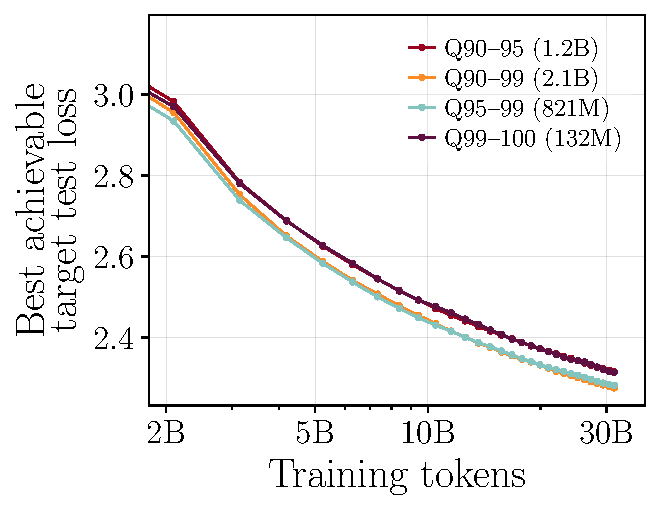
\includegraphics[width=\textwidth]{figures/paper_comparison_1x_best_loss.pdf}
      \caption{5$\times$ data scale.}
      \label{fig:quality_best_loss_1x}
  \end{subfigure}%
  \hfill
  \begin{subfigure}[t]{0.48\textwidth}
      \centering
      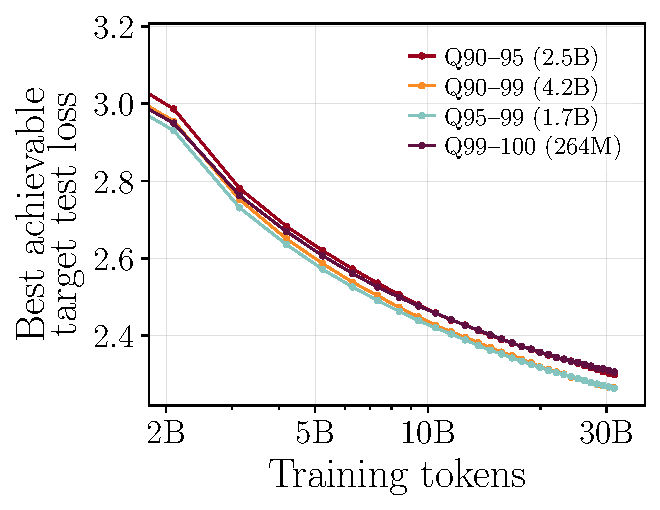
\includegraphics[width=\textwidth]{figures/paper_comparison_2x_best_loss.pdf}
      \caption{10$\times$ data scale.}
      \label{fig:quality_best_loss_2x}
  \end{subfigure}

  \caption{Best achievable target loss by quality band at (a) 5$\times$ and (b) 10$\times$ target data scales. Unlike the 1$\times$ setting (\cref{fig:comparison_best_loss}), at larger pool sizes no single quality band dominates: the curves largely overlap, confirming that the quality-quantity tradeoff diminishes when pools are large enough to avoid severe repetition.}
  \label{fig:quality_best_loss_1x_2x}
  \end{figure}


\paragraph{Experiments with overlapping buckets}
We use the full untruncated pool at each quality threshold (Q80--100: 5B, Q90--100: 2B, Q95--100: 954M, Q99--100: 132M) and train for 10B tokens.  In this expeirment, the quality bands are (e.g., all contain the Q99-100 data), representing the practical approach of setting a single lower-bound quality threshold.  The results are consistent.  The 95th percentile, Q95--100, achieves the best loss consistent with the Q95-99 results for up to 10B tokens in \Cref{fig:quality_inclusive}.

\begin{figure}[h!]
\centering
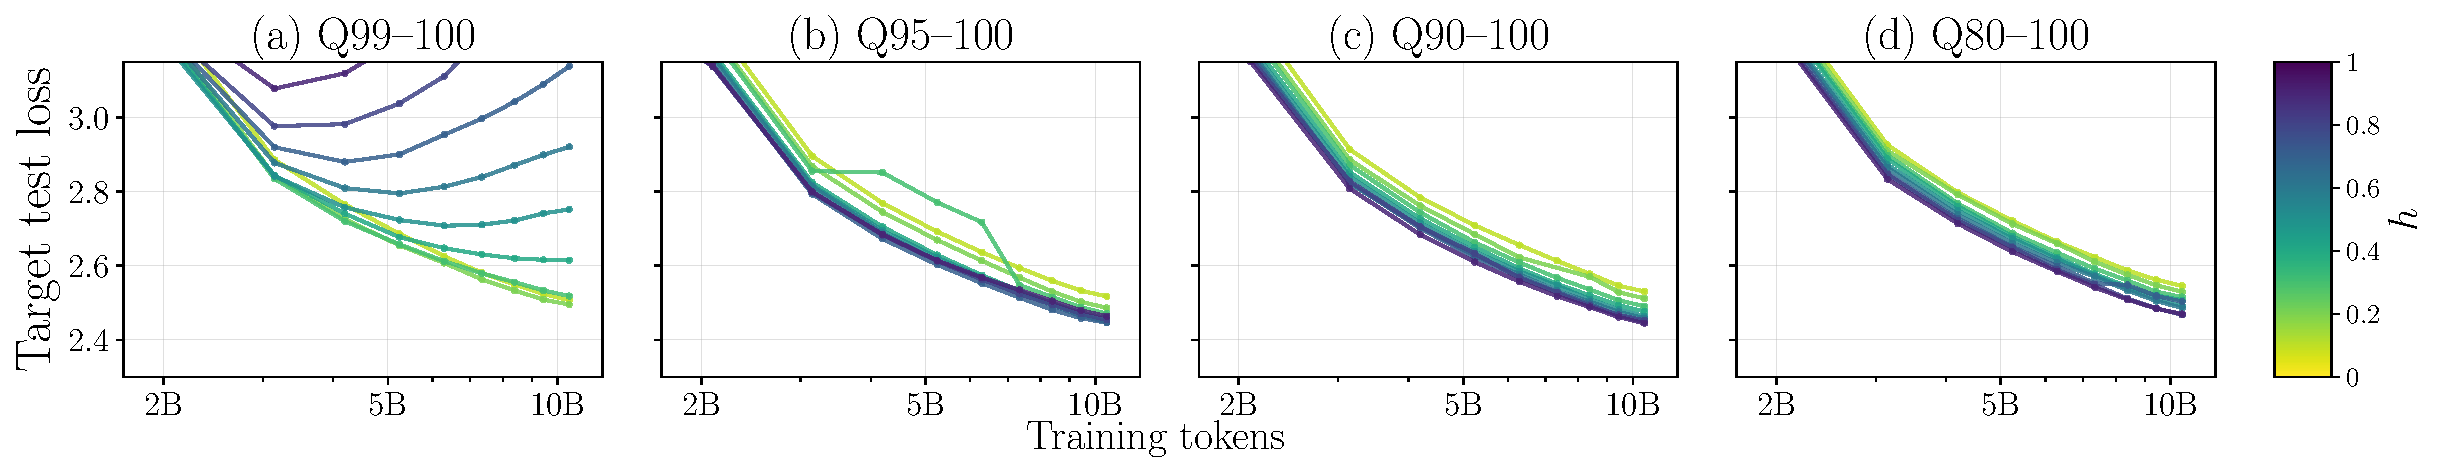
\includegraphics[width=\textwidth]{figures/paper_comparison_inclusive_combined.pdf}
\caption{Loss curves for inclusive quality thresholds (each band includes all data above the given percentile). Pool sizes increase from left to right as broader thresholds include more data.}
\label{fig:quality_inclusive}
\end{figure}


\paragraph{Equal-size data constrained size experiments.}
We truncate each quality band (Q80--100, Q90--100, Q95--100, Q99--100) to approximately the same pool size (${\sim}$132--139M tokens) and train for 10B tokens. This isolates the effect of per-token quality by controlling for pool size as all bands have approximately the same number of repetitions. \ref{fig:quality_same_pool} shows results when the data constrained pools are equal size.  With the impact of repetition equalized across quality, the ordering is strict: Q99--100 $>$ Q95--100 $>$ Q90--100 $>$ Q80--100 at all training steps.

\begin{figure}[h!]
\centering
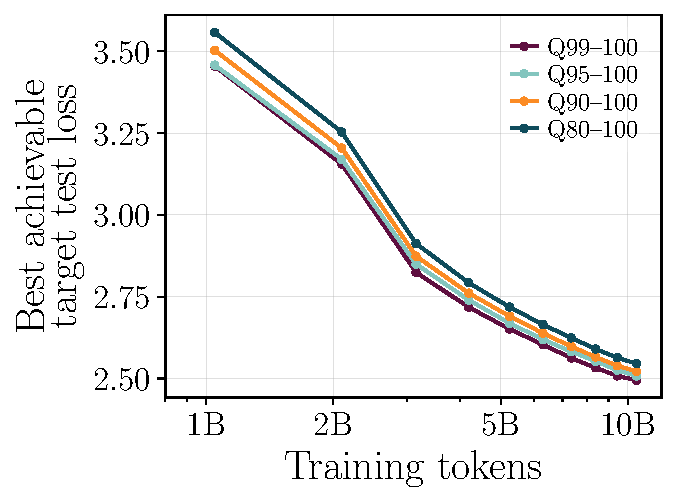
\includegraphics[width=0.45\textwidth]{figures/paper_comparison_same_pool_best_loss.pdf}
\caption{Best achievable target loss with all quality bands truncated to the same pool size. With repetition equalized, higher per-token quality consistently achieves lower loss.}
\label{fig:quality_same_pool}
\end{figure}


\paragraph{Final remarks} When pool size is equalized, quality improves validation loss.  When pools vary naturally, the repetition penalty from small high-quality pools outweighs the quality advantage. The non-overlapping band experiments isolate the mechanism: it is the data in broader bands (Q90--99 beyond Q95--99) that helps at larger training budgets, not merely reduced repetition of the top slice. The scale dependence of the crossover has a practical implication that for any given training budget and data pool, there exists an optimal quality threshold that balances per-token quality against repetition.  Our scaling law captures this tradeoff enabling practitioners to extrapolate which data pool to use and for how many repetitions.















\section{Comparison to Unlimited Target Data}
\label{app:unlimited}

To establish an upper bound on target-domain performance, we train all model sizes with a ${\sim}60$B German token pool -- large enough that repetition never occurs. Figure~\ref{fig:unlimited_all_h} shows target loss for each mixture fraction $h$ in this unlimited setting. Without data constraints, higher target fractions monotonically achieve lower target loss at every training budget: there is no overfitting, no U-shaped behavior, and no quality--quantity tradeoff. 

\begin{figure}[h!]
\centering
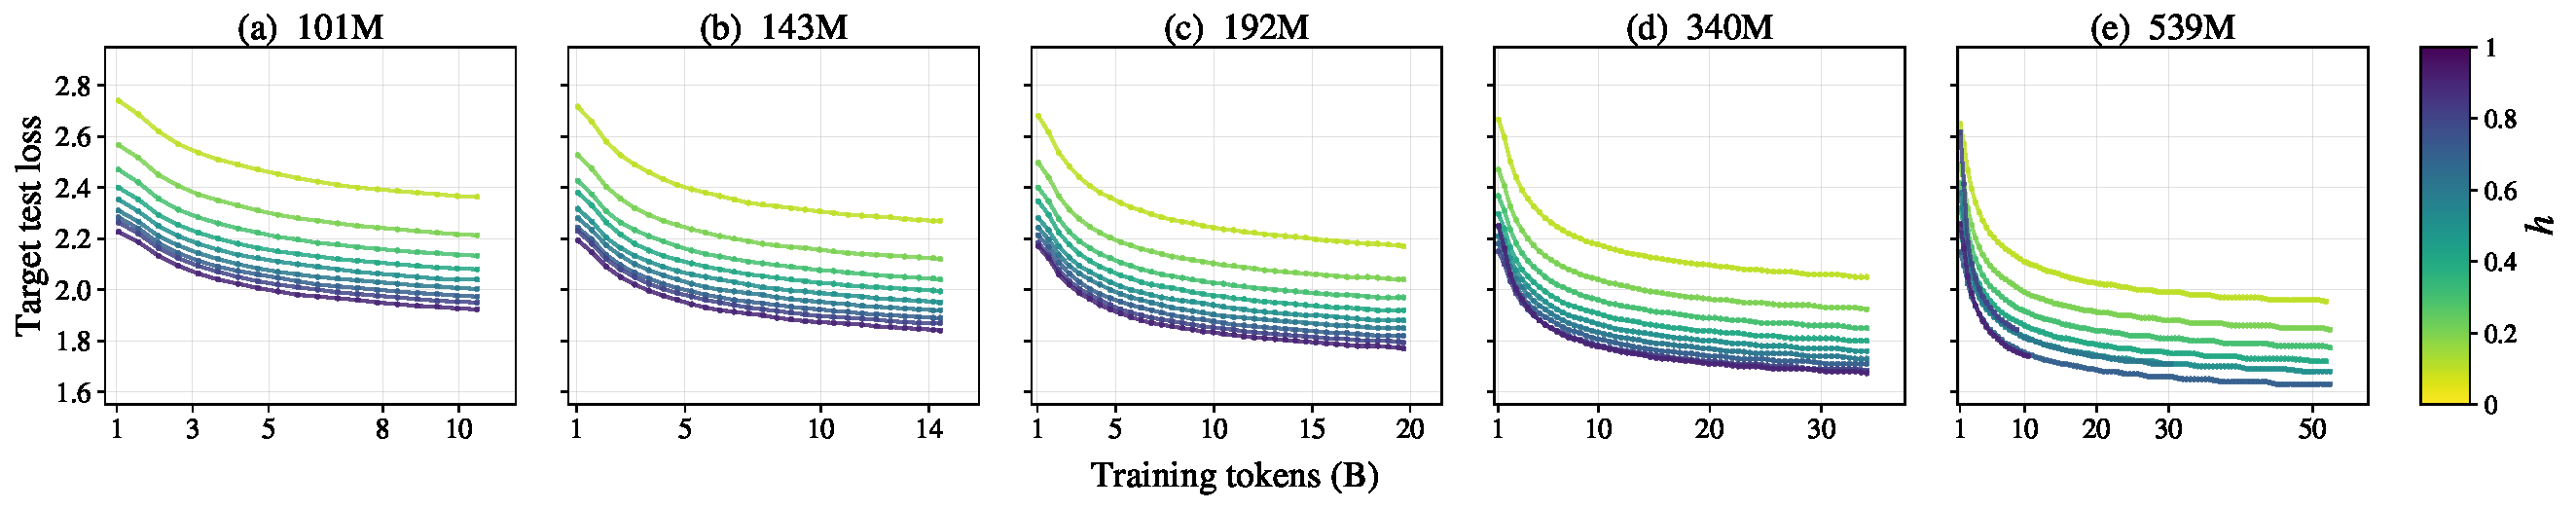
\includegraphics[width=\textwidth]{figures/paper_unlimited_all_h.pdf}
\caption{German target loss with unlimited data (${\sim}60$B pool, $r < 1$ throughout) for all mixture fractions $h$. Without data constraints, higher target fractions always achieve lower target loss, and no overfitting occurs.}
\label{fig:unlimited_all_h}
\end{figure}

Figure~\ref{fig:unlimited_comparison} then compares the best achievable loss under constrained pools (50M--1B) against this unlimited baseline. The gap between each constrained curve and the unlimited line quantifies the cost of the data constraint. Constrained pools plateau as training progresses while the unlimited baseline continues to improve, confirming that the performance ceiling is imposed by data exhaustion rather than model capacity. The gap widens with training budget, underscoring the importance of optimal mixture design when target data is scarce.

\begin{figure}[h!]
\centering
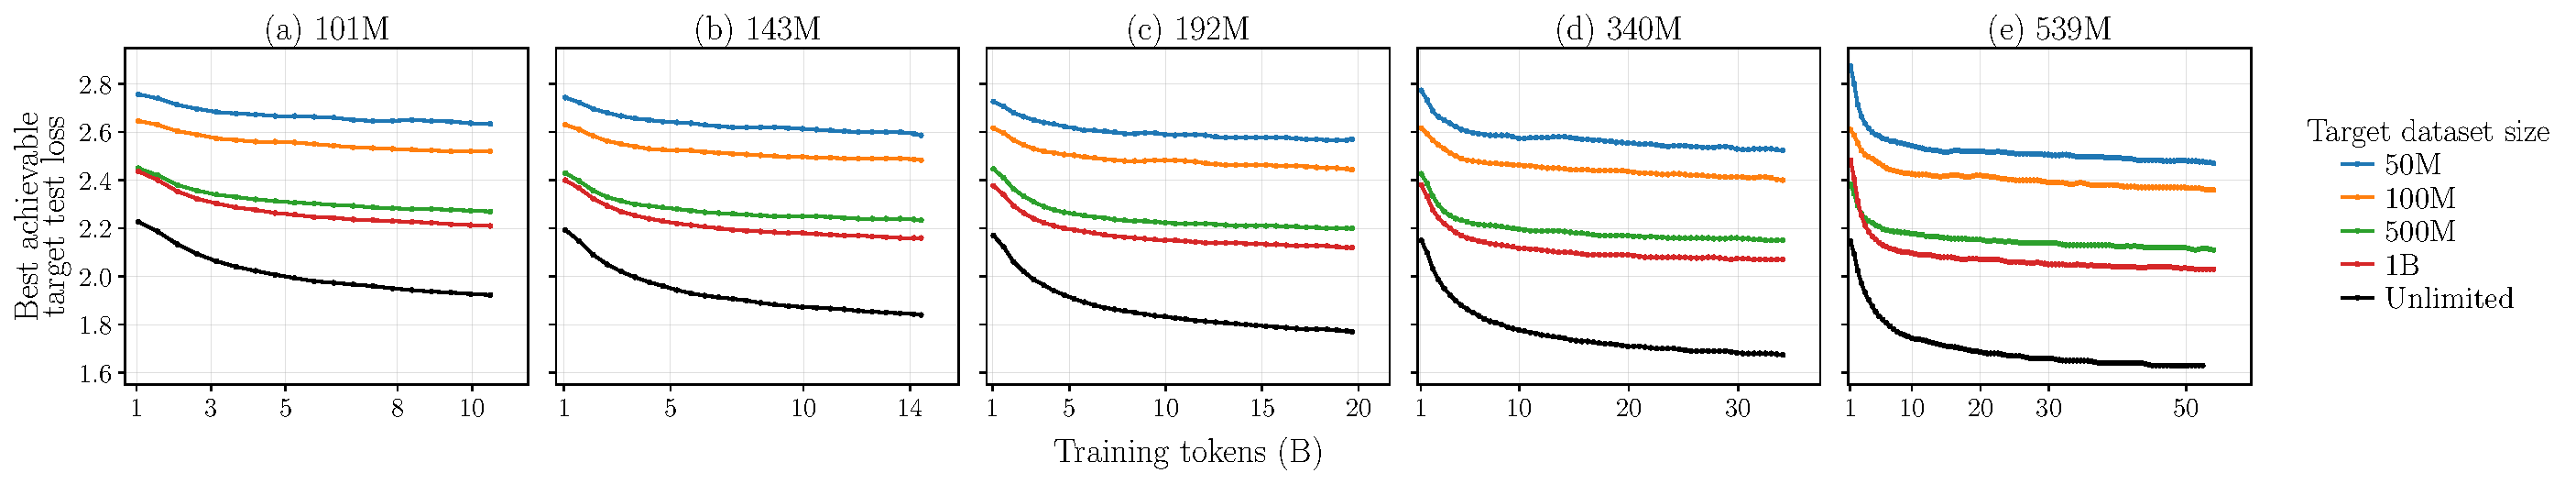
\includegraphics[width=\textwidth]{figures/paper_best_loss_vs_unlimited_all.pdf}
\caption{Best achievable German target loss vs.\ training tokens for each model size, comparing constrained data pools against an unlimited (${\sim}60$B) baseline where target data is never repeated.}
\label{fig:unlimited_comparison}
\end{figure}


\section{Analysis of Three-Domain Experiments}
\label{app:3domain}

Section~\ref{sec:multi_domain} presents results under proportional weighting; here we report the complementary equal-weighting experiments ($h_{\text{wiki}} = h_{\text{peS2o}}$).

Figure~\ref{fig:3domain_equal} shows optimal repetition under equal weighting with the 10\% compute confidence band. The core pattern from the proportional case carries over: optimal $r$ grows steadily with training budget, and smaller data pools require substantially higher repetition before the optimum is reached. Under equal weighting, the smaller domain (Wiki) is repeated more aggressively than under proportional weighting, as equal weights allocate the same weight to both domains regardless of pool size, and the smaller pool exhausts its unique tokens earlier. For example, at 10B training tokens in the base configuration (Wiki 100M, peS2o 500M), equal weighting reaches $r \approx 14$ while proportional weighting stays at $r \approx 6$ (measured with respect to the Wiki pool). The confidence bands remain wide, confirming that approximate repetition estimates suffice for near-optimal performance under either strategy.

\begin{figure}[h!]
\centering
\vspace{-10pt}
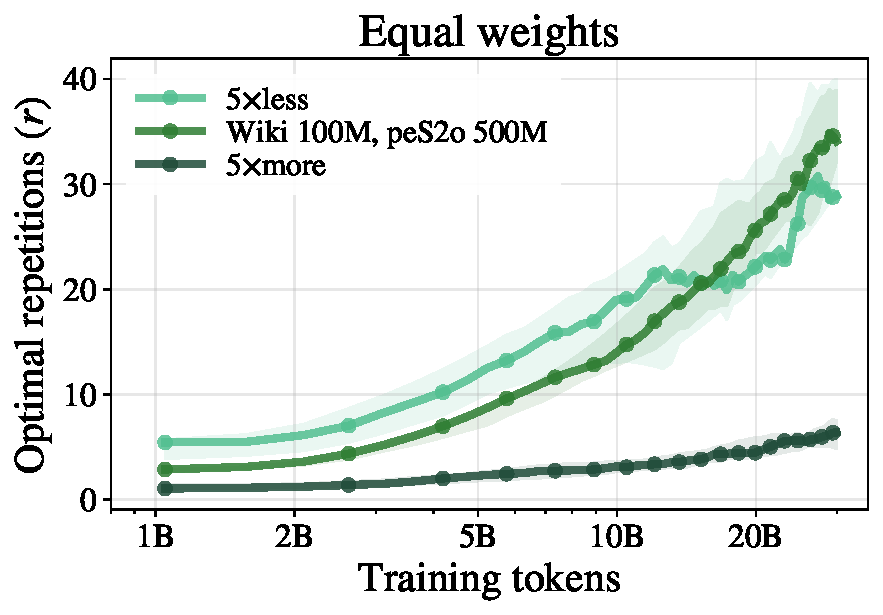
\includegraphics[width=0.45\textwidth]{figures/appendix/fig_3domain_equal_weights.pdf}
\caption{Optimal repetitions under equal weighting with 10\% compute confidence band (shaded) in the three-domain setup (101M model).}
\label{fig:3domain_equal}
\end{figure}

\begin{figure}[h!]
    \centering
    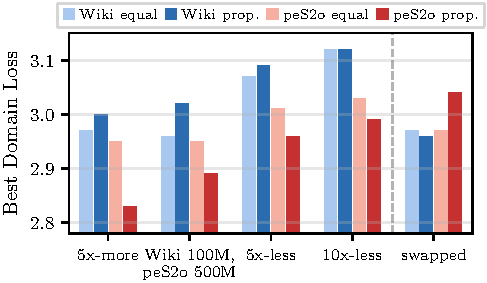
\includegraphics[width=0.55\textwidth]{figures/appendix/fig_3domain_strategy_bars.pdf}
    \caption{Per-domain best loss under equal vs.\ proportional weighting across five pool-size configurations.}
    \label{fig:3domain_bars}
    \vspace{-10pt}
\end{figure}


Additionally, we examined how the choice of weighting strategy affects each target domain individually. Beyond the configurations reported in the main text, we include a 10$\times$less experiment (Wiki 10M, peS2o 50M) to test both strategies under even more severe data constraints. Figure~\ref{fig:3domain_bars} breaks down the per-domain loss under both strategies across all five configurations. Proportional weighting consistently favors the larger pool (peS2o), achieving lower peS2o loss at the expense of Wiki. Equal weighting reverses this tradeoff: it assigns more relative weight to the smaller domain, improving Wiki loss but sacrificing peS2o performance. The effect is most pronounced when pool sizes differ substantially: in the 5$\times$more configuration, proportional weighting achieves 0.12 lower peS2o loss than equal weighting, while equal weighting gains only 0.03 on Wiki. The \emph{swapped} configuration (where Wiki becomes the larger pool) confirms this pattern: when pool sizes are reversed, proportional weighting now favors Wiki instead.




Figure~\ref{fig:3domain_optimal_loss_all} shows the best achievable per-domain loss throughout training for all four pool-size configurations.

\begin{figure}[h!]
\centering
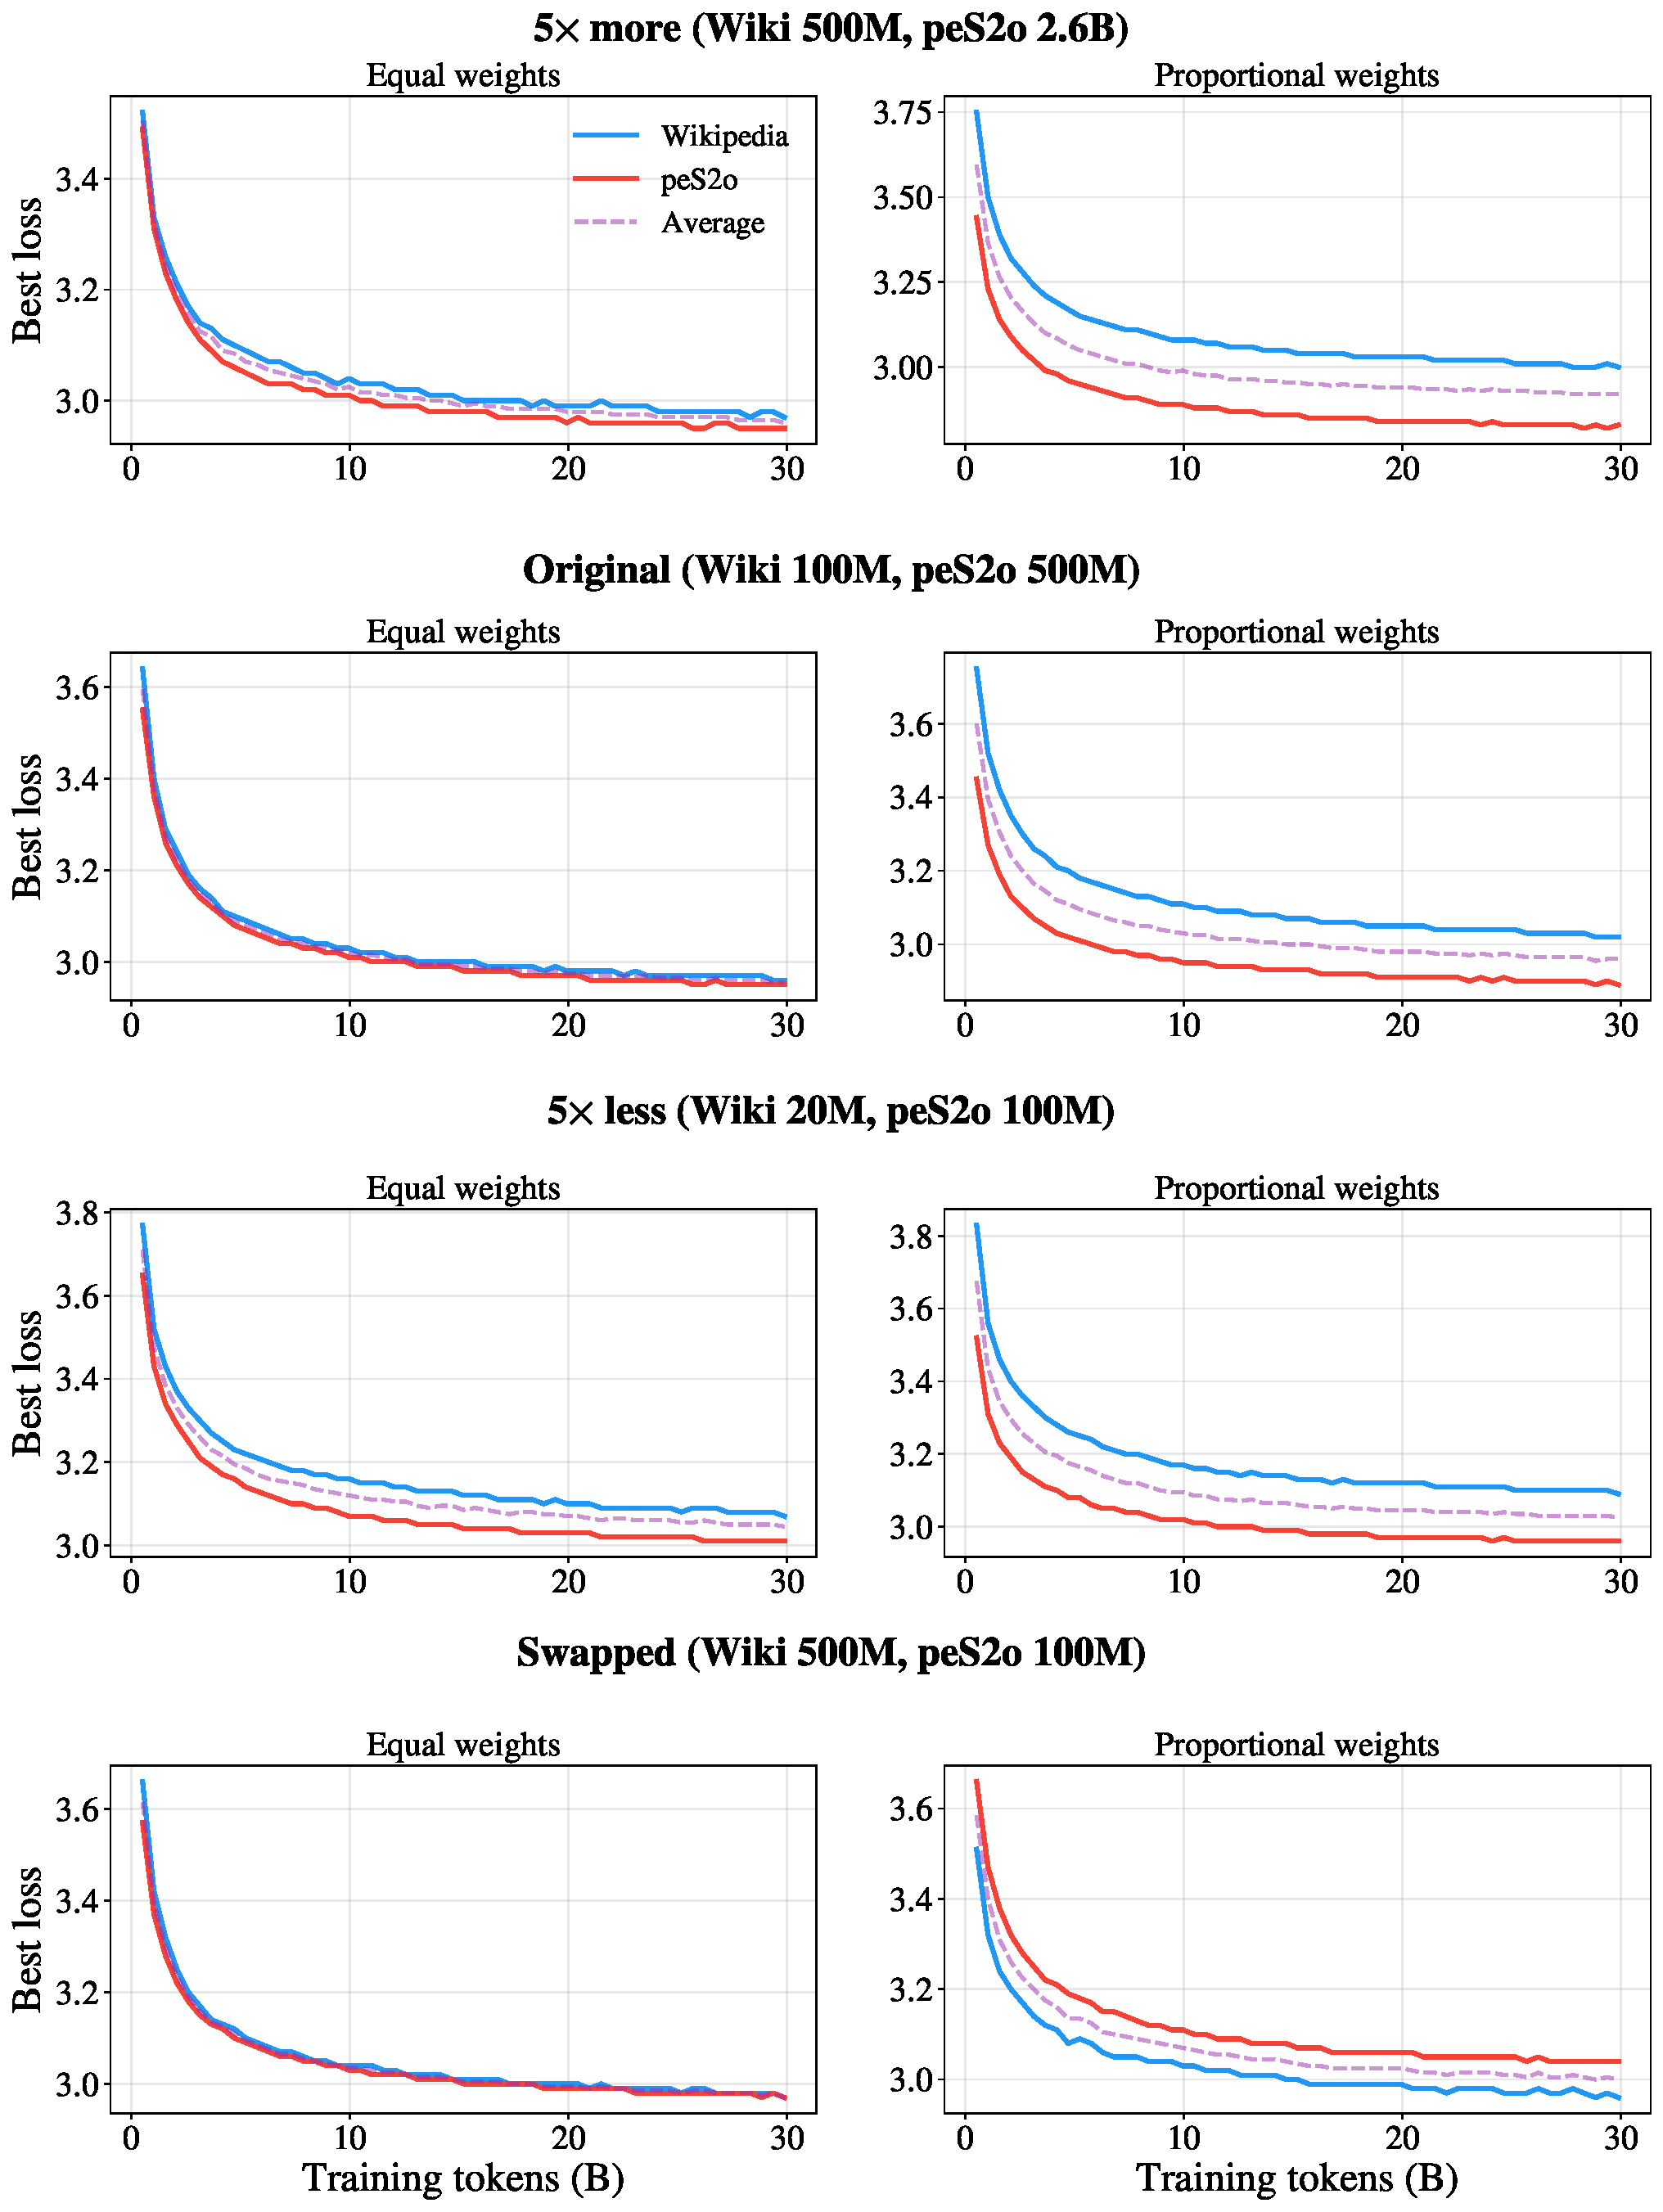
\includegraphics[width=0.65\textwidth]{figures/paper_3domain_optimal_loss_all_configs.pdf}
\caption{Best achievable per-domain loss throughout training under equal (left) and proportional (right) weighting for four pool-size configurations. Blue: Wikipedia; red: peS2o; dashed purple: average.}
\vspace{-5pt}
\label{fig:3domain_optimal_loss_all}
\end{figure}

\newpage
\section{Baseline Scaling Law Formulas}
\label{app:details}

We describe the baseline formulas used in Section~\ref{sec:scaling_results}.
All formulas predict the target-domain loss as a function of the total tokens $D_\text{total}$, the target weight $h$, the number of repetitions $r = h\,D_\text{total}/D_\text{target}$, and optionally the model size $N$.

\paragraph{Repetitions-agnostic~\citep{shukor2025scalinglawsoptimaldata}.}
This baseline treats all tokens as unique regardless of repetition:
\begin{equation}
  L = E + \frac{A}{D_\mathrm{eff}^\alpha} + \gamma\,h\,,
  \qquad D_\mathrm{eff} = (1-h)\,D_\text{total} + \tau\,h\,D_\text{total}\,.
\end{equation}
The effective data is a weighted sum of generic and target tokens with no repetition discounting---repeated target tokens are valued the same as fresh ones.
Parameters: $E$, $A$, $\alpha$, $\tau$, $\gamma$ (5 parameters).

\paragraph{Domain-agnostic~\citep{muennighoff2023scaling}.}
This baseline uses a single saturating function of total tokens without distinguishing domains:
\begin{equation}
  L = E + A\,D_\mathrm{eff}^{\,\alpha}\,,
  \qquad D_\mathrm{eff} = C\bigl(1 - e^{-\mu\,R}\bigr)\,,
\end{equation}
where $C = (1-h)\,D_\text{total} + h\,D_\text{total}/r$ is the total number of unique tokens and $R = D_\text{total}/C$ is the overall repetition ratio.
Parameters: $E$, $A$, $\alpha$ ($<0$), $\mu$ (4 parameters).

\paragraph{Utility decay~\citep{goyal2024scaling}.}
This baseline models repetition through an exponentially decaying exponent:
\begin{equation}
  L = E + a\,D_\text{total}^{\,b_\mathrm{eff}}\,,
  \qquad b_\mathrm{eff} = (1-h)\,b_0 + h\,b_1\,\delta^{r-1}\,,
\end{equation}
where $\delta = 0.5^{1/\tau}$ is a half-life parameter.
As repetitions increase, the exponent on the target-domain contribution decays toward zero, reducing the data-scaling benefit.
Parameters: $E$, $a$, $b_0$, $b_1$, $\tau$ (5 parameters).

\paragraph{Multi-size extensions.}
Each baseline extends to variable model size by adding a capacity term $C/N^\beta$ (and for the repetitions-agnostic and domain-agnostic formulas, a data-size coupling $N^\delta$), following the same pattern as $L_\mathrm{size}$ (Eq.~\ref{eq:lsize}).



\section{Extended Scaling Law Results}
\label{app:extended_scaling}

This section reports the full results underlying Section~\ref{sec:scaling_results}, including the train/test breakdown for the loss prediction tables, the per-dataset optimal-mixture prediction errors, and the size-extrapolation wasted-token metric.

\paragraph{Loss prediction: train and test $wR^2$ (fixed-size formula).}
Table~\ref{tab:app_scaling_r2_full} reports train and test $wR^2$ on all four experimental setups for the fixed-size formula $L_\mathrm{fix}$ and the three baselines. Train corresponds to the first 50\% of training steps, test to the held-out second half.

\begin{table}[h]
\centering
\caption{Train and test weighted $R^2$ ($wR^2$) for the fixed-size formula $L_\mathrm{fix}$, fitted independently per model size (or per quality level / domain). Each observation is weighted by $\max(r \cdot h, \epsilon)$ to emphasise the high-repetition regime. Train: first 50\% of steps; test: second half.}
\label{tab:app_scaling_r2_full}
\small
\begin{tabular}{lcccccccc}
\toprule
& \multicolumn{2}{c}{German} & \multicolumn{2}{c}{Maths} & \multicolumn{2}{c}{Quality} & \multicolumn{2}{c}{Wiki/peS2o} \\
\cmidrule(lr){2-3} \cmidrule(lr){4-5} \cmidrule(lr){6-7} \cmidrule(lr){8-9}
& Train & Test & Train & Test & Train & Test & Train & Test \\
\midrule
$L_\mathrm{fix}$ & \textbf{0.85} & \textbf{0.95} & \textbf{0.99} & \textbf{0.88} & \textbf{0.91} & \textbf{0.71} & 0.68 & \textbf{0.80} \\
Rep-agnostic & 0.81 & 0.78 & 0.95 & 0.78 & 0.86 & 0.14 & 0.67 & 0.72 \\
Utility decay & 0.52 & 0.72 & 0.77 & 0.55 & 0.94 & $-$0.64 & \textbf{0.69} & 0.79 \\
Domain-agnostic & 0.03 & $-$40.7 & 0.10 & $-$0.49 & 0.46 & $-$2.19 & 0.42 & $-$1.16 \\
\bottomrule
\end{tabular}
\end{table}

\paragraph{Loss prediction: train and test $wR^2$ (size extrapolation).}
Table~\ref{tab:app_scaling_r2_size_full} reports the same metric for the multi-size formula $L_\mathrm{size}$, fitted on all model sizes except the largest and evaluated on the held-out largest model.

\begin{table}[h]
\centering
\caption{Size extrapolation: weighted $R^2$ ($wR^2$) for the multi-size formula $L_\mathrm{size}$, fitted on smaller model sizes and evaluated on the held-out largest model (539M for German, 936M for Maths). Train: $wR^2$ on fitting sizes; Test: $wR^2$ on held-out size.}
\label{tab:app_scaling_r2_size_full}
\small
\begin{tabular}{lcccccc}
\toprule
& \multicolumn{2}{c}{German (539M)} & \multicolumn{2}{c}{Maths (936M)} \\
\cmidrule(lr){2-3} \cmidrule(lr){4-5}
& Train & Test & Train & Test \\
\midrule
$L_\mathrm{size}$ & \textbf{0.95} & \textbf{0.65} & \textbf{0.97} & \textbf{0.73} \\
Rep-agnostic+$N$ & 0.88 & 0.59 & 0.94 & 0.71 \\
Utility decay+$N$ & 0.76 & 0.56 & 0.85 & 0.69 \\
Domain-agnostic+$N$ & 0.25 & $-$0.23 & 0.46 & $-$0.77 \\
\bottomrule
\end{tabular}
\end{table}

\paragraph{Optimal mixture prediction error.}
For each experiment (a specific model size and target dataset size) and each held-out training checkpoint $D_\text{total}$, we compare the predicted $h^*$ to the empirically best weight $h^*_\text{emp}$ at that checkpoint. Table~\ref{tab:app_hstar_error} reports the median of $|\log_{10}(h^*_\text{pred}) - \log_{10}(h^*_\text{emp})|$ per dataset over all such pairs on held-out test steps. A value of $0.1$ corresponds to a ${\sim}1.26\times$ multiplicative error in the predicted weight.

\begin{table}[h]
\centering
\caption{Optimal mixture prediction on held-out test steps: median $|\log_{10}(h^*_\text{pred}) - \log_{10}(h^*_\text{emp})|$ (lower is better). A value of $0.1$ corresponds to a ${\sim}1.26\times$ error in the predicted fraction.}
\label{tab:app_hstar_error}
\small
\begin{tabular}{lccccc}
\toprule
& Ger. & Math & Qual. & Wiki & Avg \\
\midrule
$L_\mathrm{fix}$ & \textbf{0.07} & \textbf{0.13} & 0.47 & \textbf{0.10} & \textbf{0.19} \\
Rep-agnostic & 0.60 & 1.01 & 0.61 & 0.50 & 0.68 \\
Utility decay & 0.10 & 0.20 & \textbf{0.38} & 0.12 & 0.20 \\
Domain-agn. & 2.57 & 1.99 & 5.30 & 3.07 & 3.23 \\
\midrule
$L_\mathrm{size}$ & \textbf{0.15} & 0.18 & --- & --- & 0.17 \\
Rep-agn.+$N$ & 0.73 & 1.44 & --- & --- & 1.09 \\
Util. dec.+$N$ & \textbf{0.15} & \textbf{0.17} & --- & --- & \textbf{0.16} \\
Dom.-agn.+$N$ & 3.27 & 1.56 & --- & --- & 2.42 \\
\bottomrule
\end{tabular}
\end{table}

\paragraph{Size extrapolation: wasted tokens.}
A stronger test of the multi-size formula is whether it can predict the behaviour of a model size never seen during fitting. We fit $L_\mathrm{size}$ and all multi-size baselines on all model sizes \emph{except the largest} and evaluate exclusively on the held-out largest model (539M for German, 936M for Maths). Table~\ref{tab:size_extrap_wasted} reports the weighted median wasted token fraction on the held-out largest model for each setup.
$L_\mathrm{size}$ achieves a test $wR^2$ of $0.65$ on German and $0.73$ on Maths (Table~\ref{tab:app_scaling_r2_size_full}), demonstrating that the capacity and data-size coupling terms extrapolate meaningfully to larger scales.
The wasted token metric is even more discriminating: most baselines fail catastrophically on German, producing predictions outside the empirical range (counted as~$100\%$).
$L_\mathrm{size}$ wastes $58\%$ on German and $24\%$ on Maths, the only formula that avoids catastrophic failure on both.
Results for French and Swahili are reported in Appendix~\ref{app:size_extrap}.

\begin{table}[h]
\centering
\caption{Size extrapolation: weighted median wasted token fraction (lower is better). Predictions outside the empirical weight range are counted as $100\%$.}
\label{tab:size_extrap_wasted}
\small
\begin{tabular}{lcc}
\toprule
& German (539M) & Maths (936M) \\
\midrule
$L_\mathrm{size}$ & \textbf{58\%} & \textbf{24\%} \\
Rep-agnostic+$N$ & 100\% & 97\% \\
Utility decay+$N$ & 100\% & 22\% \\
Domain-agnostic+$N$ & 100\% & 84\% \\
\bottomrule
\end{tabular}
\end{table}


\paragraph{Limitations}
The scaling law is descriptive: it summarises observed training dynamics but does not prescribe an optimal allocation from first principles.
Size extrapolation is encouraging on both German ($wR^2 = 0.65$ at 539M) and Maths ($wR^2 = 0.73$ at 936M), though the wasted-token metric reveals that predictions remain imperfect at unseen scales.
The quality-filtering setup is harder to predict than language/domain splits (test $wR^2 = 0.71$, log-error $= 0.47$), likely because quality tiers interact with the model in ways not fully captured by the effective data abstraction.
Finally, our experiments span ${\sim}100\text{M}$--$900\text{M}$ parameters; whether the fitted exponents extrapolate to multi-billion-parameter models remains an open question.

\paragraph{Size Extrapolation: French and Swahili}
\label{app:size_extrap}

We repeat the size-extrapolation experiment of Section~\ref{sec:scaling_results} on French and Swahili.
For each language, we fit the multi-size formulas on model sizes 101M--340M and evaluate on the held-out 539M model.
Table~\ref{tab:size_extrap_app} reports weighted $R^2$ (test\,/\,train).

On French, $L_\mathrm{size}$ achieves a test $wR^2$ of $0.93$, even exceeding its train $wR^2$ of $0.92$, what indicates that the 539M model's behaviour is well predicted by trends from smaller scales.
On Swahili, extrapolation is harder: $L_\mathrm{size}$ achieves $0.69$ on the held-out 539M model, while the utility decay baseline reaches $0.71$.
The domain-agnostic baseline yields near-zero or negative $wR^2$ on both languages.

For wasted tokens, all formulas (including $L_\mathrm{size}$) produce predictions outside the empirical weight range for French and Swahili at 539M, resulting in ${\geq}94\%$ waste.
This reflects the narrower range of target fractions tested at this scale for these languages rather than a fundamental failure of the formula.

\begin{table}[h!]
\centering
\caption{Size extrapolation on French and Swahili: weighted $R^2$ (test\,/\,train) when fitting on 101M--340M and evaluating on 539M.}
\label{tab:size_extrap_app}
\begin{tabular}{lcc}
\toprule
& French (539M) & Swahili (539M) \\
\midrule
$L_\mathrm{size}$ (9p) & \textbf{0.93}\,/\,\textbf{0.92} & 0.69\,/\,\textbf{0.92} \\
Rep-agnostic+$N$ (8p) & 0.87\,/\,0.90 & 0.65\,/\,0.90 \\
Utility decay+$N$ (7p) & 0.69\,/\,0.62 & \textbf{0.71}\,/\,0.69 \\
Domain-agnostic+$N$ (7p) & $-$0.54\,/\,0.08 & $-$0.00\,/\,0.02 \\
\bottomrule
\end{tabular}
\end{table}


\section{Robustness to Weighting Scheme}
\label{app:weighting}

We verify that the qualitative ranking of formulas is robust to the choice of observation weights in the $wR^2$ metric.
Table~\ref{tab:weighting_robustness} reports test $wR^2$ on the German dataset under four weighting schemes: $\max(r \cdot h,\,\epsilon)$ (our default), $r$ only, $h$ only, and uniform (standard $R^2$).
The ranking $L_\mathrm{fix}$ $>$ rep-agnostic $>$ utility decay $>$ domain-agnostic is preserved across all schemes, confirming that the advantage of our formula is not an artifact of the weighting.
\begin{table}[h!]
\centering
\caption{Test $wR^2$ on German under different weighting schemes. The formula ranking is stable across all choices.}
\label{tab:weighting_robustness}
\begin{tabular}{lcccc}
\toprule
& $r \cdot h$ (default) & $r$ & $h$ & Uniform \\
\midrule
$L_\mathrm{fix}$ (6p) & \textbf{0.96} & \textbf{0.95} & \textbf{0.78} & \textbf{0.90} \\
Rep-agnostic (5p) & 0.81 & 0.82 & 0.52 & 0.85 \\
Utility decay (5p) & 0.78 & 0.85 & 0.39 & 0.71 \\
Domain-agnostic (4p) & $<$$-$1 & $<$$-$1 & $<$$-$1 & $<$$-$1 \\
\bottomrule
\end{tabular}
\end{table}


\section{Downstream Benchmark Evaluation}
\label{app:downstream}

We evaluate downstream task performance for the best-loss configurations from Figure~\ref{fig:diminishing} (one checkpoint per model size and data pool combination, selected at the training step that minimizes German test loss). We use seven benchmarks covering reasoning, commonsense, and language understanding:
ARC-Challenge and ARC-Easy \citep{clark2018think} (science question answering),
HellaSwag \citep{zellers2019hellaswag} (commonsense sentence completion),
LAMBADA \citep{paperno2016lambada} (long-range word prediction),
PIQA \citep{bisk2020piqa} (physical intuition reasoning),
SciQ \citep{welbl2017sciq} (science multiple-choice),
and WinoGrande \citep{sakaguchi2020winogrande} (coreference resolution).
Each benchmark is evaluated in both English (original) and German (translated), allowing us to assess both target-domain and non-target-domain capabilities from the same checkpoint.

Tables~\ref{tab:downstream_de} and~\ref{tab:downstream_en} report accuracy on all benchmarks.
German benchmark performance improves consistently with both model size and target data pool size, confirming that the perplexity gains translate to downstream improvements. English performance decreases as more training budget is allocated to German (higher $h$), reflecting the expected trade-off between target and non-target domains. Larger models partially mitigate this cost: the 539M model retains 48.6\% English average even at the highest German allocation, compared to 39.7\% for 101M.

\begin{table}[h]
\centering
\caption{German downstream benchmark accuracy (\%) at the best target-loss checkpoint. More target data consistently improves German performance across all model sizes.}
\label{tab:downstream_de}
\begin{tabular}{ll ccccccc c}
\toprule
Model & Dataset size & ARC-C & ARC-E & HSwag & Lambada & PIQA & SciQ & Wino & \textbf{Avg} \\
\midrule
101M & 50M  & 24.0 & 31.0 & 28.0 & 13.7 & 52.1 & 60.4 & 50.8 & 37.2 \\
101M & 100M & 24.5 & 31.2 & 28.4 & 15.2 & 53.0 & 63.2 & 50.2 & 37.9 \\
101M & 500M & 23.4 & 32.6 & 29.8 & 17.6 & 55.3 & 60.1 & 50.3 & 38.5 \\
101M & 1B   & 25.7 & 30.9 & 29.8 & 19.1 & 57.0 & 59.1 & 48.9 & 38.6 \\
\midrule
143M & 50M  & 23.2 & 29.9 & 28.6 & 15.3 & 52.4 & 61.7 & 50.1 & 37.3 \\
143M & 100M & 23.7 & 31.9 & 28.7 & 16.3 & 54.4 & 62.3 & 51.5 & 38.4 \\
143M & 500M & 23.7 & 33.5 & 29.8 & 19.3 & 56.5 & 63.2 & 50.8 & 39.6 \\
143M & 1B   & 24.3 & 33.1 & 30.5 & 20.7 & 56.0 & 62.8 & 50.7 & 39.7 \\
\midrule
192M & 50M  & 24.1 & 31.0 & 28.9 & 15.4 & 53.7 & 62.1 & 49.7 & 37.8 \\
192M & 100M & 24.2 & 32.7 & 29.6 & 16.9 & 53.9 & 63.2 & 50.5 & 38.7 \\
192M & 500M & 24.1 & 32.3 & 31.2 & 20.0 & 57.6 & 62.7 & 51.3 & 39.9 \\
192M & 1B   & 24.2 & 35.3 & 31.2 & 20.8 & 57.5 & 62.2 & 52.9 & 40.6 \\
\midrule
340M & 50M  & 24.2 & 31.2 & 29.2 & 15.7 & 52.8 & 62.6 & 51.4 & 38.2 \\
340M & 100M & 25.0 & 33.0 & 30.4 & 18.4 & 53.7 & 64.2 & 49.7 & 39.2 \\
340M & 500M & 24.8 & 33.8 & 32.2 & 24.1 & 57.6 & 65.3 & 53.0 & 41.5 \\
340M & 1B   & 25.3 & 36.1 & 32.9 & 24.6 & 57.2 & 64.3 & 52.5 & 41.8 \\
\midrule
539M & 50M  & 24.2 & 31.0 & 29.8 & 19.0 & 52.9 & 64.6 & 50.0 & 38.8 \\
539M & 100M & 26.1 & 31.8 & 31.6 & 19.7 & 54.7 & 65.3 & 51.5 & 40.1 \\
539M & 500M & 25.1 & 35.3 & 34.3 & 23.6 & 57.4 & 64.5 & 52.5 & 41.8 \\
539M & 1B   & 25.2 & 37.3 & 35.1 & 24.3 & 59.3 & 65.2 & 51.4 & \textbf{42.6} \\
\bottomrule
\end{tabular}
\end{table}

\begin{table}[h]
\centering
\caption{English downstream benchmark accuracy (\%) at the same checkpoints. More target data (higher $h$) reduces English performance, reflecting the trade-off between target and non-target domains.}
\label{tab:downstream_en}
\begin{tabular}{ll ccccccc c}
\toprule
Model & Pool & ARC-C & ARC-E & HSwag & Lambada & PIQA & SciQ & Wino & \textbf{Avg} \\
\midrule
101M & 50M  & 23.1 & 40.2 & 32.9 & 31.4 & 64.7 & 62.7 & 50.7 & 43.7 \\
101M & 100M & 23.1 & 40.2 & 32.6 & 30.8 & 64.9 & 65.3 & 49.8 & 43.8 \\
101M & 500M & 21.3 & 35.3 & 28.8 & 24.6 & 61.6 & 57.8 & 51.5 & 40.1 \\
101M & 1B   & 21.8 & 35.5 & 28.0 & 22.5 & 60.7 & 57.8 & 51.5 & 39.7 \\
\midrule
143M & 50M  & 23.2 & 40.4 & 34.6 & 36.6 & 65.2 & 64.0 & 50.5 & 44.9 \\
143M & 100M & 24.6 & 41.2 & 34.9 & 32.5 & 66.5 & 67.7 & 51.0 & 45.5 \\
143M & 500M & 23.3 & 38.8 & 32.2 & 29.9 & 64.6 & 66.0 & 48.9 & 43.4 \\
143M & 1B   & 22.4 & 38.9 & 30.3 & 28.8 & 63.0 & 62.8 & 51.9 & 42.6 \\
\midrule
192M & 50M  & 24.7 & 41.3 & 37.9 & 35.5 & 67.3 & 66.6 & 51.9 & 46.4 \\
192M & 100M & 23.9 & 41.3 & 36.8 & 35.8 & 67.7 & 67.4 & 51.2 & 46.3 \\
192M & 500M & 23.4 & 41.0 & 35.0 & 32.0 & 65.8 & 66.1 & 50.7 & 44.9 \\
192M & 1B   & 22.1 & 38.6 & 31.3 & 29.4 & 63.0 & 62.7 & 51.8 & 42.7 \\
\midrule
340M & 50M  & 24.2 & 45.2 & 41.9 & 39.8 & 68.9 & 69.7 & 52.9 & 48.9 \\
340M & 100M & 24.3 & 44.6 & 42.3 & 40.6 & 69.2 & 69.9 & 51.2 & 48.9 \\
340M & 500M & 25.4 & 44.2 & 40.1 & 40.0 & 68.5 & 70.1 & 51.7 & 48.6 \\
340M & 1B   & 24.3 & 42.3 & 38.5 & 38.5 & 66.2 & 67.6 & 51.3 & 47.0 \\
\midrule
539M & 50M  & 26.4 & 46.6 & 46.5 & 45.4 & 70.3 & 71.4 & 52.8 & \textbf{51.3} \\
539M & 100M & 24.7 & 47.5 & 46.5 & 45.4 & 69.5 & 72.4 & 53.7 & 51.4 \\
539M & 500M & 24.6 & 46.6 & 45.2 & 43.1 & 69.2 & 70.1 & 52.4 & 50.2 \\
539M & 1B   & 24.3 & 45.4 & 42.3 & 42.1 & 67.5 & 69.0 & 49.7 & 48.6 \\
\bottomrule
\end{tabular}
\end{table}

\newpage
\section{Limitations}
\label{sec:limitations}
We did not tune training hyperparameters jointly with the mixture and repetition settings, instead using standard values throughout. It is possible that interactions between learning rate, batch size, or schedule and the number of repetitions could shift the optimal operating points we report.
Additionally, all experiments use a single architecture family (GPT-2-style decoder-only transformers); whether the observed scaling behavior transfers to other architectures remains an open question. We leave both explorations to future work.
Our largest model is 939M parameters; while we observe consistent trends across model sizes suggesting the scaling law extrapolates, verifying this at scales of tens or hundreds of billions of parameters would require substantially more compute than available for this study.

